% !TeX program = pdflatex
% !TeX encoding = UTF-8
% OVERLEAF: selecione monografia.tex como documento principal; compilador pdfLaTeX.
% Exige as imagens da pasta figuras/. Não usa arquivos .bib nem estilos locais.
%
% Normas de referência:
% - ABNT NBR 14724:2024: apresentação de trabalhos acadêmicos.
% - ABNT NBR 6024:2012: numeração progressiva das seções.
% - ABNT NBR 6027:2012: sumário.
% - ABNT NBR 6028:2021: resumos e palavras-chave.
% - ABNT NBR 10520:2023: citações. Nas citações entre parênteses, os sobrenomes ficam em
%   maiúsculas, como pede o modelo da FATEC.
% - ABNT NBR 6023:2025: referências.
%
% A formatação segue o modelo de Trabalho de Graduação da FATEC de São José dos Campos
% (Professor Jessen Vidal): A4, fonte Times de 12 pontos, margens superior/esquerda de 3 cm e
% inferior/direita de 2 cm e entrelinha 1,5.
% Fontes para consulta:
% https://ctan.org/pkg/abntex2
% https://biblioteca.ufes.br/normalizacao

\documentclass[
  12pt,
  oneside,
  a4paper,
  chapter=TITLE,
  sumario=tradicional,
  english,
  brazil
]{abntex2}

% Codificação, fonte com suporte a acentos e recursos básicos.
\usepackage[T1]{fontenc}
\usepackage[utf8]{inputenc}
\usepackage{newtxtext}
\usepackage{newtxmath}
\usepackage{microtype}
\usepackage{graphicx}
\usepackage{booktabs}
\usepackage{longtable}

% Margens e parágrafos.
\setlrmarginsandblock{3cm}{2cm}{*}
\setulmarginsandblock{3cm}{2cm}{*}
\checkandfixthelayout
\OnehalfSpacing
\setlength{\parindent}{1.25cm}
\setlength{\parskip}{0pt}
\frenchspacing

% Títulos alinhados à esquerda, com ponto depois do número ("1. INTRODUÇÃO", "1.1. Título").
% Capítulos em maiúsculas (opção chapter=TITLE), negrito e 14 pt. Subitens em negrito e 12 pt.
\renewcommand{\ABNTEXchapterfont}{\normalfont\bfseries}
\renewcommand{\ABNTEXchapterfontsize}{\fontsize{14}{17}\selectfont}
\renewcommand{\ABNTEXsectionfont}{\normalfont\bfseries}
\renewcommand{\ABNTEXsectionfontsize}{\normalsize}
\renewcommand{\ABNTEXsubsectionfont}{\normalfont\bfseries}
\renewcommand{\ABNTEXsubsectionfontsize}{\normalsize}
\setsecnumdepth{subsection}
\setsecnumformat{\csname the#1\endcsname.\quad}
\makeatletter
\renewcommand{\printchapternum}{%
  \tocprintchapter
  \setboolean{abntex@innonumchapter}{false}%
  \chapnumfont
  \space\thechapter
  \ifthenelse{\boolean{abntex@apendiceousecao}}{\space\tocinnonumchapter\ABNTEXcaptiondelim}{.\space}%
}
\makeatother

% Sumário com recuo por nível, capítulos em maiúsculas e negrito e ponto depois de cada número.
% Nos apêndices e anexos, o travessão separa a letra do título.
\renewcommand{\cftchapteraftersnum}{.}
\renewcommand{\cftsectionaftersnum}{.}
\renewcommand{\cftsubsectionaftersnum}{.}
\makeatletter
\settocpreprocessor{chapter}{%
  \let\tempf@rtoc\f@rtoc
  \def\f@rtoc{\texorpdfstring{\MakeTextUppercase{\tempf@rtoc}}{\tempf@rtoc}}}
\makeatother
\cftinsertcode{A}{\renewcommand{\cftchapteraftersnum}{\space\textendash\space}}
\renewcommand{\tocpartapendices}{\cftinserthook{toc}{A}}
\renewcommand{\tocpartanexos}{\cftinserthook{toc}{A}}

% Cabeçalho só com o número da página, em 10 pt, no canto superior direito.
\makeevenhead{abntheadings}{}{}{\ABNTEXfontereduzida\thepage}
\makeoddhead{abntheadings}{}{}{\ABNTEXfontereduzida\thepage}
\makeheadrule{abntheadings}{\textwidth}{0pt}

% Fonte de 10 pt para a fonte e as notas das ilustrações e para as citações longas.
\renewcommand{\ABNTEXfontereduzida}{\fontsize{10}{12}\selectfont}
\setlength{\ABNTEXcitacaorecuo}{4cm}

% Legendas acima da figura ou da tabela, centralizadas, em negrito e terminadas em ponto.
\captionnamefont{\bfseries}
\captiontitlefont{\bfseries}
\captionstyle{\centering}
\captiontitlefinal{.}

% A fonte e as notas usam o mecanismo da legenda, mas ficam à esquerda, sem negrito e sem o ponto
% final da legenda.
\makeatletter
\renewcommand{\fonte}[2][\fontename]{%
  \M@gettitle{#2}%
  \memlegendinfo{#2}%
  \par
  \begingroup
    \@parboxrestore
    \if@minipage\@setminipage\fi
    \ABNTEXfontereduzida
    \captionnamefont{\normalfont}\captiontitlefont{\normalfont}%
    \captionstyle{\raggedright}\captiontitlefinal{}%
    \captiondelim{\ABNTEXcaptionfontedelim}%
    \@makecaption{\ABNTEXfontereduzida #1}{\ignorespaces\ABNTEXfontereduzida #2}\par
  \endgroup}
\makeatother

% Dados do trabalho: substituir os campos entre colchetes.
% Título provisório. Ajustar depois dos resultados da campanha.
\titulo{Custo do TreeSHAP em um sistema de detecção de intrusão em rede:
  estratégias de explicação, latência e cobertura}
\autor{Pedro Felipe Sousa Garcia}
\local{São José dos Campos}
\data{2026}
\orientador[Orientador:]{Prof. Me. José Walmir Gonçalves Duque}
\instituicao{Faculdade de Tecnologia de São José dos Campos: Professor Jessen Vidal}
\tipotrabalho{Trabalho de Graduação}
\preambulo{Trabalho de Graduação apresentado à Faculdade de Tecnologia de São José dos Campos,
  como parte dos requisitos necessários para a obtenção do título de Tecnólogo em Análise e
  Desenvolvimento de Sistemas.}

% Capa e folha de rosto conforme o modelo da FATEC: autor e título em maiúsculas e negrito,
% instituição no topo da capa e orientador à direita na folha de rosto.
\renewcommand{\imprimircapa}{%
  \begin{capa}%
    \center
    {\bfseries FACULDADE DE TECNOLOGIA DE SÃO JOSÉ DOS CAMPOS\par
    FATEC PROFESSOR JESSEN VIDAL\par}
    \vfill
    {\bfseries\MakeTextUppercase{\imprimirautor}\par}
    \vfill
    \begin{center}
      \bfseries\large\MakeTextUppercase{\imprimirtitulo}
    \end{center}
    \vfill
    \imprimirlocal\par
    \imprimirdata
    \vspace*{1cm}
  \end{capa}%
}
\renewcommand{\folhaderostocontent}{%
  \begin{center}
    {\bfseries\MakeTextUppercase{\imprimirautor}\par}
    \vspace*{\fill}
    {\bfseries\large\MakeTextUppercase{\imprimirtitulo}\par}
    \vspace*{\fill}
    \hspace{.45\textwidth}
    \begin{minipage}{.5\textwidth}
      \SingleSpacing
      \imprimirpreambulo
    \end{minipage}%
    \vspace*{\fill}
  \end{center}
  \begin{flushright}
    \textbf{\imprimirorientadorRotulo~\imprimirorientador}
  \end{flushright}
  \vspace*{\fill}
  \begin{center}
    \imprimirlocal\par
    \imprimirdata
  \end{center}
}

\hypersetup{
  hidelinks,
  pdftitle={Custo do TreeSHAP em um sistema de detecção de intrusão em rede},
  pdfauthor={Pedro Felipe Sousa Garcia},
  pdfsubject={Trabalho de Graduação}
}

\addto\captionsbrazil{\renewcommand{\listfigurename}{Lista de figuras}}

% Termo definido no Glossário: itálico com link para o verbete.
\newcommand{\termo}[2]{\hyperref[gl:#1]{\emph{#2}}}

\begin{document}
\selectlanguage{brazil}

% ---------------------------------------------------------------------------
% Elementos pré-textuais
% ---------------------------------------------------------------------------
\pretextual

\imprimircapa
\imprimirfolhaderosto*

% Verso da folha de rosto: dados de catalogação, referência bibliográfica e cessão de direitos.
\begin{fichacatalografica}
  \setlength{\parindent}{0pt}
  \textbf{Dados Internacionais de Catalogação-na-Publicação (CIP)}\\
  \textbf{Divisão de Informação e Documentação}

  \vspace{0.3cm}
  \fbox{\begin{minipage}{\dimexpr\textwidth-2\fboxsep-2\fboxrule\relax}
    \setlength{\parindent}{0pt}
    \vspace{0.2cm}
    GARCIA, Pedro Felipe Sousa\\
    \imprimirtitulo.\\
    \imprimirlocal, \imprimirdata.\\
    \thelastsheet\ f.

    \vspace{0.3cm}
    Trabalho de Graduação -- Curso de Tecnologia em Análise e Desenvolvimento de Sistemas.\\
    FATEC de São José dos Campos: Professor Jessen Vidal, \imprimirdata.\\
    Orientador Interno ou Principal: \imprimirorientador.

    \vspace{0.3cm}
    1. Detecção de intrusão. 2. Inteligência artificial explicável. 3. TreeSHAP. 4. Latência.
    5. CIC-IDS2017. I. Faculdade de Tecnologia. FATEC de São José dos Campos: Professor Jessen
    Vidal. Divisão de Informação e Documentação. II. Título.
    \vspace{0.2cm}
  \end{minipage}}

  \vspace{1cm}
  \textbf{REFERÊNCIA BIBLIOGRÁFICA}

  \vspace{0.3cm}
  GARCIA, Pedro Felipe Sousa. \textbf{\imprimirtitulo}. \imprimirdata. \thelastsheet\ f.
  Trabalho de Graduação -- FATEC de São José dos Campos: Professor Jessen Vidal.

  \vspace{1cm}
  \textbf{CESSÃO DE DIREITOS}

  \vspace{0.3cm}
  NOME DO AUTOR: \imprimirautor\\
  TÍTULO DO TRABALHO: \imprimirtitulo\\
  TIPO DO TRABALHO/ANO: Trabalho de Graduação/\imprimirdata.

  \vspace{0.3cm}
  É concedida à FATEC de São José dos Campos: Professor Jessen Vidal permissão para reproduzir
  cópias deste Trabalho e para emprestar ou vender cópias somente para propósitos acadêmicos e
  científicos. O autor reserva outros direitos de publicação e nenhuma parte deste Trabalho pode
  ser reproduzida sem a autorização do autor.

  \vspace{1.5cm}
  \rule{7cm}{0.4pt}\\
  \imprimirautor

  \vspace{0.5cm}
  São José dos Campos - SP
\end{fichacatalografica}

% Folha de aprovação conforme o modelo da FATEC: banca, orientador e data da aprovação.
\begin{folhadeaprovacao}
  \begin{center}
    {\bfseries\MakeTextUppercase{\imprimirautor}\par}
    \vspace*{\fill}
    {\bfseries\large\MakeTextUppercase{\imprimirtitulo}\par}
    \vspace*{\fill}
    \hspace{.45\textwidth}
    \begin{minipage}{.5\textwidth}
      \SingleSpacing
      \imprimirpreambulo
    \end{minipage}%
    \vspace*{\fill}
  \end{center}

  \setlength{\ABNTEXsignwidth}{14cm}
  \assinatura{\textbf{Prof. Me. Antonio Egydio São Thiago Graça -- FATEC}}
  \assinatura{\textbf{Prof. Me. Carlos Henrique Loureiro Feichas -- FATEC}}
  \assinatura{\textbf{\imprimirorientador{} -- FATEC}}

  \vspace*{\fill}
  \begin{center}
    \rule{1.2cm}{0.4pt}/\rule{1.2cm}{0.4pt}/\rule{1.2cm}{0.4pt}\par
    \vspace{0.3cm}
    DATA DA APROVAÇÃO
  \end{center}
\end{folhadeaprovacao}

% \begin{dedicatoria}
%   \vspace*{\fill}
%   \begin{flushright}
%     \textit{[TODO: texto da dedicatória.]}
%   \end{flushright}
% \end{dedicatoria}

\begin{agradecimentos}

Não sei se seria melhor começar pelo princípio ou pelo fim. Supondo que o mais comum seja começar
pelo início, me esforçarei em começar pelo fim.

O fim é este documento, que ninguém lê com mais atenção que a banca. Nem mesmo o autor,
com a caneta na mão e a concentração do escritor, consegue ler como um juiz. Por isso,
os agradecimentos iniciais chegam aos componentes da banca, que não satisfeitos com esta página,
precisarão chegar à última. Mas tranquilizem-se. Apenas aqui eu tomo a liberdade do estilo.

Por orientar este TG com a paciência de quem já viu muito deploy de sexta-feira,
agradeço ao Prof. Me. José Walmir Gonçalves Duque.

Foram seis semestres de FATEC, e faltaria papel à impressora para falar sobre todos os professores
que me ensinaram, com dedicação e paciência, a ser um bom profissional. A todos eles, deixo meus agradecimentos.

Aos colegas que dividiram comigo esses semestres, agradeço, sobretudo, pelas discussões.
Seria prosaico e frívolo agradecê-los pela companhia; por isso, o omito. O que eu não posso omitir
são as discordâncias, as novas abordagens a problemas e soluções que eu pensava já conhecer.
A eles vai meu apreço particular por pessoas inteligentes que discordam de mim.

E, encerrando pelo princípio, agradeço àqueles que, por mais que não soubessem bem o que eu fazia,
deram-me uma vida em que trabalhos como este fossem possíveis. Esse início é a minha família, à qual devo todos os outros inícios.

\end{agradecimentos}

\begin{epigrafe}
  \vspace*{\fill}
  \begin{flushright}
    \textit{``All models are wrong, but some are useful.''}

    (George Box)
  \end{flushright}
\end{epigrafe}

\begin{resumo}
  Sistemas de detecção de intrusão em rede baseados em aprendizado de máquina classificam fluxos de
  tráfego, mas suas decisões são difíceis de interpretar. O TreeSHAP explica cada classificação de
  modelos de árvores pela contribuição de cada atributo, ao custo de um cálculo adicional por fluxo.
  Este trabalho mede esse custo num sistema de detecção de intrusão em rede (NIDS) com Random Forest e
  XGBoost, treinados com o Improved CIC-IDS2017, e compara quatro estratégias de explicação: sem
  explicação, síncrona total, síncrona condicional e assíncrona. O NIDS forma os mesmos fluxos dos
  dados de treino, marca o instante de cada etapa de cada fluxo e roda numa rede emulada pelo Mininet.
  A carga cresce com cópias simultâneas de um trecho de captura, cada uma com endereços próprios, o que
  preserva as entradas dos fluxos. Em chamadas isoladas, a explicação de um fluxo
  levou em média 7,4~ms no Random Forest e 0,43~ms no XGBoost, contra 4,9~ms e 0,18~ms da inferência.
  Com 1, 2 e 4 cópias, o XGBoost manteve a latência de classificação abaixo
  de 1~s no p95 e de 2~s no p99 em todas as estratégias, inclusive explicando todos os fluxos antes da
  entrega, salvo numa execução com perda de pacotes. No Random Forest, explicar todos os fluxos só foi
  viável na estratégia assíncrona com 1 cópia. A estratégia condicional não acrescentou latência
  mensurável, mas explicou no máximo 2,8\% dos fluxos. A viabilidade depende do custo do TreeSHAP no
  classificador e da carga.

  \vspace{\onelineskip}
  \noindent\textbf{Palavras-chave:} detecção de intrusão; inteligência artificial explicável;
  TreeSHAP; latência; CIC-IDS2017.
\end{resumo}

\begin{resumo}[Abstract]
  \begin{otherlanguage*}{english}
    Machine learning-based network intrusion detection systems classify traffic flows, but their
    decisions are hard to interpret. TreeSHAP explains each classification of tree-based models by the
    contribution of each feature, at the cost of an additional computation per flow. This work measures
    this cost in a network intrusion detection system (NIDS) with Random Forest and XGBoost, trained on
    Improved CIC-IDS2017, and compares four explanation strategies: no explanation, fully synchronous,
    conditional synchronous and asynchronous. The NIDS builds the same flows as the training data,
    records the instant of each stage of each flow and runs on a network emulated with Mininet. The load
    grows with simultaneous copies of a capture segment, each with its own addresses, which preserves
    the flow inputs. In isolated calls, explaining one flow took on average 7.4~ms with Random Forest
    and 0.43~ms with XGBoost, against 4.9~ms and 0.18~ms for inference. With 1, 2 and 4 copies, XGBoost
    kept the p95 classification latency below 1~s and the p99 below 2~s under all strategies, including
    when explaining every flow before delivery, except in one run with packet loss. With Random Forest,
    explaining every flow was feasible only with the asynchronous strategy and 1 copy. The conditional
    strategy added no measurable latency, but explained at most 2.8\% of the flows. Feasibility depends
    on the load and on the cost of TreeSHAP for the classifier.

    \vspace{\onelineskip}
    \noindent\textbf{Keywords:} intrusion detection; explainable artificial intelligence;
    TreeSHAP; latency; CIC-IDS2017.
  \end{otherlanguage*}
\end{resumo}

\pdfbookmark[0]{\listfigurename}{lof}
\listoffigures*
\cleardoublepage

\pdfbookmark[0]{\listtablename}{lot}
\listoftables*
\cleardoublepage

\begin{siglas}
  \item[ACK] \emph{Acknowledgment}
  \item[CPU] \emph{Central Processing Unit}
  \item[CSV] \emph{Comma-Separated Values}
  \item[CWR] \emph{Congestion Window Reduced}
  \item[ECE] \emph{Explicit Congestion Notification Echo}
  \item[FIN] \emph{Finish}
  \item[FTP] \emph{File Transfer Protocol}
  \item[ICMP] \emph{Internet Control Message Protocol}
  \item[ID3] \emph{Iterative Dichotomiser 3}
  \item[IP] \emph{Internet Protocol}
  \item[IPv4] \emph{Internet Protocol version 4}
  \item[LIME] \emph{Local Interpretable Model-agnostic Explanations}
  \item[NIDS] \emph{Network Intrusion Detection System}
  \item[p95] Percentil 95
  \item[p99] Percentil 99
  \item[PCAP] \emph{Packet Capture}
  \item[PSH] \emph{Push}
  \item[RF] Random Forest
  \item[ROC-AUC] \emph{Area Under the Receiver Operating Characteristic Curve}
  \item[RST] \emph{Reset}
  \item[SHAP] \emph{SHapley Additive exPlanations}
  \item[SYN] \emph{Synchronize}
  \item[TCP] \emph{Transmission Control Protocol}
  \item[UDP] \emph{User Datagram Protocol}
  \item[URG] \emph{Urgent}
  \item[UTC] \emph{Coordinated Universal Time}
  \item[XAI] \emph{Explainable Artificial Intelligence}
\end{siglas}

\pdfbookmark[0]{\contentsname}{toc}
\tableofcontents*
\cleardoublepage

% ---------------------------------------------------------------------------
% Elementos textuais
% ---------------------------------------------------------------------------
\textual

\chapter{Introdução}
\label{cap:introducao}

Um sistema de detecção de intrusão em rede (NIDS) procura ameaças no tráfego de uma rede. Ele emite
alertas quando o tráfego corresponde à assinatura de um ataque conhecido ou foge do comportamento
normal (ZUECH; KHOSHGOFTAAR; WALD, 2015). Num NIDS baseado em aprendizado de máquina, os pacotes
podem ser agrupados em \termo{fluxo}{fluxos}. Cada fluxo é descrito por atributos como a duração, o
tamanho dos pacotes e o intervalo entre pacotes. Um \termo{classificador}{classificador} treinado em
tráfego rotulado atribui, então, uma classe a cada fluxo a partir desses atributos. O CIC-IDS2017 é
um dataset público para avaliar sistemas de detecção de intrusão, que descreve por 80 atributos os
fluxos de um tráfego capturado numa rede de laboratório (SHARAFALDIN; HABIBI LASHKARI; GHORBANI,
2018). Este trabalho usa o Improved CIC-IDS2017, uma versão do CIC-IDS2017 em que erros de formação
dos fluxos, de extração de atributos e de rotulagem foram corrigidos (Seção~\ref{sec:fluxos}).

Os fluxos descritos por atributos formam dados tabulares, um tipo de dado em que modelos de árvores, como o Random Forest
(BREIMAN, 2001) e o XGBoost (CHEN; GUESTRIN, 2016), têm bom desempenho. No CIC-IDS2017, o ID3 e o
Random Forest tiveram os dois maiores valores de F1 (Seção~\ref{sec:medidas-deteccao}) entre os
algoritmos avaliados pelos autores do dataset (SHARAFALDIN; HABIBI LASHKARI; GHORBANI, 2018). Em
comparações com vários datasets tabulares, o XGBoost superou modelos de aprendizado profundo
recentes propostos para esse tipo de dado e exigiu menos ajuste de hiperparâmetros (SHWARTZ-ZIV;
ARMON, 2022).

O Random Forest e o XGBoost, porém, combinam muitas árvores de decisão. Em modelos com muitas
árvores, o relato do caminho de decisão não ajuda a explicar uma previsão (LUNDBERG et al., 2020).
Num NIDS, a opacidade do classificador dificulta ao analista de segurança validar alertas,
investigar falsos positivos e entender detecções perdidas, como Ogunseyi et al. (2026) observam em
modelos de aprendizado profundo. A inteligência artificial explicável (XAI) trata desse problema
com técnicas que explicam as decisões de um modelo (ADADI; BERRADA, 2018). Entre essas técnicas, o
TreeSHAP calcula, para cada previsão de um modelo de árvores, a contribuição de cada atributo. A
soma das contribuições com um \termo{valor-referencia}{valor de referência} reproduz a saída
explicada. O TreeSHAP reduz o cálculo exato dos valores de Shapley de tempo exponencial para tempo
polinomial no número de folhas e na profundidade das árvores (LUNDBERG et al., 2020).

Mesmo em tempo polinomial, o cálculo do TreeSHAP é uma segunda operação por fluxo, além da
inferência. Num NIDS, essa operação pode atrasar a entrega da classificação, encher filas e, em
\termo{carga}{carga} alta, fazer o sistema descartar fluxos. A literatura, porém, mede pouco esse
custo. Segundo a revisão sistemática de Ogunseyi et al. (2026), dos 129 estudos de detecção de
intrusão com aprendizado profundo explicável analisados, apenas 12 relatam alguma métrica de
eficiência. Nenhum desses estudos compara quantitativamente a latência antes e depois da
explicação.

Os trabalhos recentes sobre a latência de detecção e o custo das explicações medem o TreeSHAP em
chamadas isoladas, definem a latência de detecção sem incluir a explicação ou tratam o custo das
explicações com valores simulados (Seções~\ref{sec:latencia-nids} e~\ref{sec:relacionados}).
Nenhum desses trabalhos mede, num NIDS sob carga
controlada, a \termo{latencia-classificacao}{latência de classificação} e a
\termo{latencia-explicacao}{latência de explicação} de cada fluxo em
\termo{estrategia}{estratégias de explicação} diferentes.

Este trabalho pergunta se é viável gerar explicações TreeSHAP das classificações durante a operação
de um NIDS baseado em aprendizado de máquina, sem que a latência de classificação ultrapasse os
limites do experimento. Esses limites são de 1~s no percentil 95 (p95) e de 2~s no percentil 99
(p99) da latência de classificação, fixados no \termo{piloto}{piloto} (Seção~\ref{sec:matriz}). A hipótese tem
duas partes. A primeira é que a explicação acrescenta um custo que varia com a estratégia de
explicação e com a carga. A segunda é que explicar só alguns fluxos, ou explicar fora do
\termo{caminho}{caminho da classificação}, isto é, sem que a entrega da classificação espere pela
explicação, reduz esse custo, com custos diferentes em latência, uso de recursos e
\termo{cobertura-explicativa}{cobertura explicativa}. Para testar a hipótese, o trabalho compara
quatro estratégias de explicação num NIDS com Random Forest e XGBoost, numa rede emulada, sob
\termo{nivel-carga}{níveis de carga} controlados.

\section{Objetivos do trabalho}

O objetivo geral deste trabalho é medir o custo de gerar explicações TreeSHAP das classificações
durante a operação de um NIDS baseado em aprendizado de máquina, em latência, uso de recursos e \termo{cobertura-explicativa}{cobertura
explicativa}, sob \termo{nivel-carga}{níveis de carga} controlados. Para atingi-lo, foram estabelecidos os objetivos
específicos abaixo:
\begin{itemize}
  \item Treinar e avaliar \termo{classificador}{classificadores} Random Forest e XGBoost com o Improved CIC-IDS2017.
  \item Implementar um NIDS que classifique cada \termo{fluxo}{fluxo} e gere a explicação TreeSHAP da classificação
  nas quatro \termo{estrategia}{estratégias de explicação}.
  \item Emular uma rede que reproduza o tráfego em níveis de carga controlados, sem
  alterar as entradas dos fluxos.
  \item Medir, em cada estratégia e nível de carga, a \termo{latencia-classificacao}{latência de classificação}, a \termo{latencia-explicacao}{latência de
  explicação}, o uso de recursos, os \termo{descarte}{descartes} e a cobertura explicativa.
  \item Determinar em que combinações de classificador, estratégia e nível de carga a explicação é
  viável.
\end{itemize}

\section{Conteúdo do trabalho}

O Capítulo~\ref{cap:fundamentacao} apresenta o CIC-IDS2017 e a formação dos \termo{fluxo}{fluxos}, as
medidas de desempenho de detecção, as árvores de decisão, o Random Forest e o XGBoost, os valores de
Shapley e o TreeSHAP, a latência num NIDS e os trabalhos relacionados. O
Capítulo~\ref{cap:metodologia} descreve a arquitetura do sistema, os dados, os
\termo{classificador}{classificadores}, a configuração do TreeSHAP, o NIDS, as
\termo{estrategia}{estratégias de explicação}, o ambiente emulado, a matriz experimental e as
medidas e a disponibilidade do código e dos arquivos de saída. O
Capítulo~\ref{cap:resultados} apresenta e discute os resultados, e o Capítulo~\ref{cap:conclusao}
responde à pergunta nos limites do experimento e aponta as contribuições e os trabalhos futuros.
Em cada seção, a primeira ocorrência de cada termo definido no Glossário aparece em itálico, com
um link para o verbete.

\chapter{Fundamentação técnica}
\label{cap:fundamentacao}

\section{O CIC-IDS2017 e a formação dos fluxos}
\label{sec:fluxos}

O CIC-IDS2017 reúne cinco dias de tráfego de uma rede de laboratório, com tráfego benigno gerado a
partir do comportamento de usuários e ataques de sete famílias (SHARAFALDIN; HABIBI LASHKARI;
GHORBANI, 2018). Os \termo{fluxo}{fluxos} do dataset e seus atributos vêm do CICFlowMeter, um
extrator de atributos de fluxos distribuído pelo mesmo instituto que criou o dataset. O
CICFlowMeter lê os pacotes de uma captura em formato PCAP (\emph{Packet Capture}), o formato de
arquivo em que as ferramentas de captura de tráfego gravam cada pacote de uma interface de rede com
o instante da captura. Em seguida, ele agrupa num fluxo os pacotes com os mesmos endereços, portas
e protocolo e calcula 80 atributos de cada fluxo (Apêndice~\ref{ap:atributos}), como a duração, os intervalos entre pacotes e as
estatísticas de cada sentido da comunicação (SHARAFALDIN; HABIBI LASHKARI; GHORBANI, 2018).

O CIC-IDS2017 original, porém, tem erros. Engelen, Rimmer e Joosen (2021) encontraram erros na
geração do tráfego, na formação dos fluxos, na extração de atributos e na rotulagem do dataset. Eles
corrigiram o extrator, refizeram a extração e marcaram como \emph{Attempted} os fluxos de ataque
que não exibem comportamento malicioso. Liu et al. (2022) fizeram novas correções no extrator e
publicaram a versão usada neste trabalho, o Improved CIC-IDS2017.

No CICFlowMeter corrigido, um fluxo termina por tempo limite, por um encerramento TCP seguido de
uma nova conexão, por um pacote ICMP com código e tipo diferentes do código e do tipo do fluxo ou
no fim da captura (ENGELEN, 2022). Esse modo de encerramento atrasa a classificação num NIDS que usa
os mesmos atributos dos dados de treino, porque esse NIDS só pode classificar um fluxo depois que o
fluxo termina. Pelo tempo limite, essa espera pode chegar a 120~s depois do primeiro pacote do fluxo
(ENGELEN, 2022).

\section{Medidas de desempenho de detecção}
\label{sec:medidas-deteccao}

As medidas de desempenho de detecção comparam a classe que o
\termo{classificador}{classificador} atribui a cada registro com o rótulo do registro. O
classificador calcula a probabilidade de ataque de cada registro. O
\termo{limiar-classificacao}{limiar de classificação} é o valor dessa probabilidade acima do qual o
classificador atribui a classe ataque (FAWCETT, 2006). Neste trabalho, o limiar de classificação é 0,5
(Seção~\ref{sec:classificadores}). Ataque é a classe positiva.
Benigno é a classe negativa. Cada registro classificado pertence a um de quatro casos. Um verdadeiro
positivo (VP) é um registro de ataque classificado como ataque. Um falso positivo (FP) é um registro
benigno classificado como ataque. Um verdadeiro negativo (VN) é um registro benigno classificado
como benigno. Um falso negativo (FN) é um registro de ataque classificado como benigno, ou seja, um
ataque não detectado. Os quatro casos formam a matriz de confusão do classificador (FAWCETT, 2006),
apresentada na Tabela~\ref{tab:matriz-confusao}.

\begin{table}[htbp]
  \centering
  \caption{Matriz de confusão}
  \label{tab:matriz-confusao}
  \begin{tabular}{lll}
    \toprule
    & \multicolumn{2}{c}{Rótulo do registro} \\
    \cmidrule(lr){2-3}
    Classe atribuída & Ataque & Benigno \\
    \midrule
    Ataque & VP (verdadeiro positivo) & FP (falso positivo) \\
    Benigno & FN (falso negativo) & VN (verdadeiro negativo) \\
    \bottomrule
  \end{tabular}
  \fonte{Elaborada pelo autor com base em Fawcett (2006).}
\end{table}


A acurácia é a proporção de registros classificados corretamente, $(\mathrm{VP}+\mathrm{VN})/(\mathrm{VP}+\mathrm{FP}+\mathrm{VN}+\mathrm{FN})$. Como
75,93\% dos registros do Improved CIC-IDS2017 são benignos (Seção~\ref{sec:dados}), um
classificador que atribuísse a classe benigno a todos os registros teria acurácia próxima de 0,76
sem detectar nenhum ataque. Por isso, este trabalho também usa medidas que separam os falsos
positivos dos falsos negativos. A precisão, $\mathrm{VP}/(\mathrm{VP}+\mathrm{FP})$, é a proporção de registros de ataque
entre os registros classificados como ataque. O recall, $\mathrm{VP}/(\mathrm{VP}+\mathrm{FN})$, é a proporção dos registros
de ataque classificados como ataque. A taxa de falsos positivos, $\mathrm{FP}/(\mathrm{FP}+\mathrm{VN})$, é a proporção dos
registros benignos classificados como ataque. O F1, que Fawcett (2006) chama de \emph{F-measure}, é a média
harmônica entre a precisão $P$ e o recall $R$, $2PR/(P+R)$. Como a média harmônica fica próxima do menor dos dois valores, o F1 só é
alto quando a precisão e o recall são altos.

Essas cinco medidas dependem do limiar de classificação. A curva ROC (\emph{Receiver Operating
Characteristic}), ao contrário, considera todos os limiares e mostra o recall em função da taxa de falsos positivos quando o limiar varia de 0 a
1. A ROC-AUC é a área sob a curva ROC. Ela vale 1 quando algum limiar separa todos os registros de
ataque de todos os registros benignos e 0,5 quando a probabilidade de ataque não distingue as duas
classes (FAWCETT, 2006).

Este trabalho usa o F1 na validação para escolher a configuração de cada classificador
(Seção~\ref{sec:classificadores}) e apresenta as seis medidas no conjunto de teste
(Capítulo~\ref{cap:resultados}).

\section{Árvores de decisão, Random Forest e XGBoost}
\label{sec:arvores}

Os dois \termo{classificador}{classificadores} deste trabalho combinam árvores de decisão. Uma
árvore de decisão classifica um \termo{fluxo}{fluxo} por uma sequência de testes. Cada nó interno
compara um atributo do fluxo com um valor de corte e envia o fluxo a um de dois ramos, conforme o
resultado da comparação. O fluxo desce da raiz até um nó sem ramos, a folha, que guarda o valor de
saída da árvore para todos os fluxos que a alcançam (CHEN; GUESTRIN, 2016). A profundidade de uma
árvore é o maior número de testes entre a raiz e uma folha. Como cada nó interno tem dois ramos, uma
árvore de profundidade $D$ tem no máximo $2^D$ folhas.

O Random Forest combina muitas árvores treinadas de forma independente (BREIMAN, 2001). Duas fontes
de aleatoriedade diferenciam as árvores. Cada árvore é treinada com registros de treino sorteados
com reposição. Em cada nó, o teste é escolhido entre um subconjunto de atributos sorteado para
aquele nó. Essa aleatoriedade busca reduzir a correlação entre as árvores sem reduzir a força de cada árvore,
isto é, a sua capacidade de classificar corretamente. Como o limite superior do erro de
generalização do Random Forest cresce com essa correlação e diminui com essa força, a aleatoriedade
melhora a acurácia do Random Forest (BREIMAN, 2001). Na formulação original, o Random Forest escolhe a classe que recebe mais votos das
árvores (BREIMAN, 2001). A implementação do scikit-learn, usada neste trabalho, faz, porém, a média
das probabilidades de ataque dadas pelas árvores no lugar da votação (SCIKIT-LEARN DEVELOPERS, [2026]).
Numa árvore, a probabilidade de ataque é a proporção de registros de ataque entre os
registros de treino que chegaram à folha, de modo que a saída do Random Forest já é uma probabilidade.

O XGBoost também combina árvores, mas as treina em sequência (CHEN; GUESTRIN, 2016). Para treinar
cada nova árvore, o XGBoost usa uma função de perda, que mede a diferença entre a previsão do
classificador e o rótulo de um registro de treino. Cada nova árvore é ajustada para minimizar a soma
dessa função nos registros de treino, a partir das previsões das árvores anteriores, com um termo de
regularização que penaliza a complexidade da árvore (CHEN; GUESTRIN, 2016). Chen e Guestrin (2016) definem a saída do
XGBoost para um fluxo como a soma dos valores das folhas que o fluxo alcança em todas as árvores.
A implementação da biblioteca acrescenta a essa soma um valor inicial, comum a todos os fluxos, o
\texttt{base\_score}, que a biblioteca estima antes do treino (XGBOOST DEVELOPERS, [2026]). O \emph{shrinkage} reduz a influência de cada árvore, porque multiplica os valores das folhas
de cada nova árvore por um fator $\eta$, de 0,1 neste
trabalho (CHEN; GUESTRIN, 2016). O objetivo logístico binário
define a função de perda do XGBoost neste trabalho e trata a saída,
isto é, o valor inicial somado aos valores das folhas, como um escore na escala de log-odds, o logaritmo da razão $p/(1-p)$, em que $p$ é a probabilidade de
ataque. A função logística converte esse escore na probabilidade de ataque (XGBOOST DEVELOPERS, [2026]).

O número de árvores, o número de folhas e a profundidade, definidos nesta seção, determinam o custo
do TreeSHAP (Seção~\ref{sec:treeshap}).

\section{Valores de Shapley e TreeSHAP}
\label{sec:treeshap}

Os valores de Shapley vêm da teoria dos jogos cooperativos e repartem o resultado de um jogo entre
os jogadores (SHAPLEY, 1953). A contribuição marginal de um jogador é a mudança no resultado quando
ele entra num grupo de jogadores. O valor de Shapley de cada jogador é a média dessa contribuição
marginal sobre todas as ordens em que os jogadores podem entrar (LUNDBERG et al., 2020). Na previsão
de um \termo{classificador}{classificador}, os jogadores são os atributos da entrada
explicada, e o resultado é a saída do classificador para essa entrada. Antes de qualquer atributo
entrar, a saída é o \termo{valor-referencia}{valor de referência}, a saída esperada do classificador
quando nenhum atributo é conhecido (LUNDBERG et al., 2020). Neste trabalho, a contribuição de um atributo para a
saída explicada é o seu valor de Shapley.

A Tabela~\ref{tab:shapley} mostra o cálculo num exemplo com dois atributos, A e B. O valor de
referência é 0,2. A saída é 0,5 quando só A é conhecido, 0,3 quando só B é conhecido e 0,9 quando
os dois são conhecidos. Na ordem em que A entra antes de B, A acrescenta 0,3 à saída e B acrescenta
0,4. Na ordem inversa, B acrescenta 0,1 e A acrescenta 0,6. A média das duas ordens dá a A o valor
de Shapley de 0,45 e a B o de 0,25. O valor de referência somado aos dois valores de Shapley,
$0{,}2 + 0{,}45 + 0{,}25$, reproduz a saída de 0,9.

\begin{table}[htbp]
  \centering
  \caption{Exemplo de cálculo dos valores de Shapley com dois atributos}
  \label{tab:shapley}
  \begin{tabular}{lcc}
    \toprule
    Ordem de entrada & Contribuição marginal de A & Contribuição marginal de B \\
    \midrule
    A, depois B & $0{,}5 - 0{,}2 = 0{,}3$ & $0{,}9 - 0{,}5 = 0{,}4$ \\
    B, depois A & $0{,}9 - 0{,}3 = 0{,}6$ & $0{,}3 - 0{,}2 = 0{,}1$ \\
    \midrule
    Média (valor de Shapley) & 0,45 & 0,25 \\
    \bottomrule
  \end{tabular}
  \fonte{Elaborada pelo autor.}
  \nota{Valores ilustrativos. A saída do classificador é 0,2 sem atributos conhecidos (valor de
  referência), 0,5 só com A, 0,3 só com B e 0,9 com A e B.}
\end{table}

Essa soma corresponde à primeira de três propriedades que, entre os métodos que atribuem uma
contribuição a cada atributo, só os valores de Shapley satisfazem (LUNDBERG; LEE, 2017; LUNDBERG et
al., 2020). Pela acurácia local (\emph{local accuracy}), as contribuições somadas ao valor de
referência reproduzem a saída explicada. Pela consistência (\emph{consistency}), se o classificador
mudar de modo que o efeito de um atributo sobre a saída aumente ou se mantenha, independentemente
dos demais atributos, o valor de Shapley desse atributo não diminui. Pela ausência de efeito
(\emph{missingness}), um atributo sem efeito sobre a saída recebe contribuição nula.

O cálculo exato desses valores é exponencial no número de atributos (LUNDBERG et al., 2020). O
exemplo da Tabela~\ref{tab:shapley} usa quatro saídas, uma para cada subconjunto de atributos
conhecidos. Com $M$ atributos, são $2^M$ subconjuntos. Para cada um, o cálculo precisa da saída do
classificador quando só os atributos do subconjunto são conhecidos. Com os 80 atributos deste
trabalho, seriam $2^{80}$ subconjuntos. O TreeSHAP, que Lundberg et al. (2020) chamam de Tree SHAP, é
o algoritmo que calcula exatamente os valores de Shapley de modelos de árvores. O nome vem do SHAP
(\emph{SHapley Additive exPlanations}), o conjunto de métodos de explicação proposto por Lundberg e
Lee (2017). Em vez de enumerar os subconjuntos de atributos, o TreeSHAP percorre a estrutura das
árvores, o que reduz o custo a $O(TLD^2)$, em que $T$ é o número de árvores, $L$ o maior número
de folhas de uma árvore e $D$ a maior profundidade (LUNDBERG et al., 2020).

As duas variantes do TreeSHAP diferem no tratamento dos atributos desconhecidos. Na variante
\emph{path-dependent}, num nó que testa um atributo desconhecido, o cálculo segue os dois ramos e
pondera cada ramo pela proporção dos registros de treino que seguiram por esse ramo, medida pela
\termo{cobertura-no}{cobertura do nó}. Como essa informação fica guardada nas próprias árvores,
o cálculo dispensa um \termo{conjunto-referencia}{conjunto de referência} (LUNDBERG et al., 2020). Na
variante \emph{interventional}, o cálculo substitui cada atributo desconhecido pelo seu valor em
cada registro de um conjunto de referência e faz a média das saídas, de modo que o custo cresce com
o tamanho desse conjunto (LUNDBERG et al., 2020).

\section{Latência num NIDS}
\label{sec:latencia-nids}

Dash e Acken (2026) tratam a latência de detecção como a rapidez com que um sistema de detecção de
intrusão identifica as intrusões. Eles observam que os trabalhos da área a definem de modos
diferentes, como \termo{tempo-inferencia}{tempo de inferência}, tempo de comunicação ou tempo de
computação, o que torna os resultados incomparáveis. A definição que propõem soma três componentes,
a latência controlada pelo atacante, a latência determinada pelo sistema de detecção e a latência
posterior à detecção. A segunda componente é decomposta em partes que dependem da topologia da rede
e do método de detecção.

Como essa definição não inclui a explicação, este trabalho mede três tempos por
\termo{fluxo}{fluxo} dentro do NIDS. O tempo de inferência é a duração da chamada ao
\termo{classificador}{classificador}. A \termo{latencia-classificacao}{latência de classificação}
vai do fim da extração dos atributos do fluxo ao momento em que a classificação fica disponível a
quem a consome. A \termo{latencia-explicacao}{latência de explicação} vai do mesmo instante, o fim
da extração dos atributos, ao momento em que a explicação fica disponível. A diferença entre a
latência de classificação de uma \termo{estrategia}{estratégia de explicação} e a latência de
classificação sem explicação, sob a mesma \termo{carga}{carga} e o mesmo classificador, é a
\termo{sobrecarga}{sobrecarga de latência} da estratégia.

A Tabela~\ref{tab:tempos-fluxo} mostra esses tempos para um fluxo em três das estratégias de
explicação da Seção~\ref{sec:estrategias}. O fluxo espera 3~ms antes de chegar ao \termo{processo-classificador}{processo classificador}, a
inferência leva 5~ms e a explicação, 7~ms. No \termo{sem-xai}{Sem XAI}, a classificação é entregue
sem explicação, e a latência de classificação é de 8~ms. No \termo{sincrono-total}{Síncrono total},
a classificação só é entregue depois da explicação, de modo que a latência de classificação e a
latência de explicação são de 15~ms e a sobrecarga de latência é de 7~ms. No
\termo{assincrono}{Assíncrono}, a classificação é entregue aos 8~ms, e o pedido de explicação
espera 10~ms numa fila antes de ser atendido. A latência de explicação chega a 25~ms, mas a latência
de classificação não muda, e a sobrecarga de latência é nula neste exemplo.

\begin{table}[htbp]
  \centering
  \caption{Exemplo dos tempos de um fluxo em três estratégias de explicação, em milissegundos}
  \label{tab:tempos-fluxo}
  \begin{tabular}{lcccc}
    \toprule
    Estratégia & \begin{tabular}[c]{@{}c@{}}Tempo de\\inferência\end{tabular} & \begin{tabular}[c]{@{}c@{}}Latência de\\classificação\end{tabular} &
    \begin{tabular}[c]{@{}c@{}}Latência de\\explicação\end{tabular} & \begin{tabular}[c]{@{}c@{}}Sobrecarga\\de latência\end{tabular} \\
    \midrule
    Sem XAI & 5 & $3 + 5 = 8$ & --- & --- \\
    Síncrono total & 5 & $3 + 5 + 7 = 15$ & 15 & $15 - 8 = 7$ \\
    Assíncrono & 5 & $3 + 5 = 8$ & $8 + 10 + 7 = 25$ & $8 - 8 = 0$ \\
    \bottomrule
  \end{tabular}
  \fonte{Elaborada pelo autor.}
  \nota{Valores ilustrativos: 3~ms de espera antes do processo classificador, 5~ms de inferência, 7~ms de
  explicação e, no Assíncrono, 10~ms de espera na fila de explicações pendentes.}
\end{table}

\section{Trabalhos relacionados}
\label{sec:relacionados}

Bertoli et al. (2020) mostram que o desempenho de um \termo{classificador}{classificador} medido no
sistema em funcionamento difere do medido sobre o dataset. Eles treinaram uma árvore de decisão
sobre 12 atributos do cabeçalho TCP/IP para detectar varreduras TCP e a implementaram como módulo
do núcleo do Linux num Raspberry Pi, com o tráfego de ataque passando pelo sistema. A árvore de
profundidade 11, com F1 de 0,96 na análise do dataset, detectou 68\% dos ataques avaliados no
sistema. A de profundidade 6, com F1 de 0,92, detectou 82\%. Este trabalho adota a mesma avaliação
de ponta a ponta e a estende ao custo das explicações, que Bertoli et al. não medem.

Nugraha, Jnanashree e Bauschert (2025) propõem um arcabouço de detecção explicável em duas etapas.
A primeira etapa combina um teste estatístico com a importância global dos atributos calculada pelo
SHAP e mantém os dez atributos mais informativos. A segunda etapa treina um classificador XGBoost e
explica cada decisão com SHAP e LIME, comparando as duas explicações. A avaliação usa três
datasets, entre eles o CICIoT2023, e mede o tempo de cada explicação sobre registros desses
datasets, numa estação de trabalho com AMD Ryzen 7 3800X. O TreeSHAP levou de 0,02~s a 0,08~s por
explicação. No ataque SYN Flood, o LIME levou 36,38~s com todos os atributos e 9,48~s com os dez
atributos escolhidos. Esses tempos medem cada explicação isolada, fora de um sistema que recebe
tráfego.

Le et al. (2026) tratam a explicação como um serviço com custo num NIDS com recursos limitados. O
mecanismo que propõem escolhe entre sete ações de explicação, como suprimir, adiar, gerar a
explicação local completa ou transferi-la para outro nível da rede. A escolha depende, entre outros
fatores, da pressão de pacotes, da dívida de explicações e de um orçamento de exposição. A dívida de
explicações cresce quando explicações são adiadas ou geradas com menos detalhe e pesa mais para os
alertas de maior risco. O orçamento de exposição limita quanto as explicações liberadas revelam
sobre as fronteiras de decisão do classificador e diminui a cada explicação liberada (LE et al.,
2026). A avaliação usa processos de chegada sintéticos ou reproduzidos e sequências de escores
calibradas em três datasets. Nela, o custo de cada ação é um peso relativo, normalizado a partir de
medições num equipamento comum, e não uma latência medida num NIDS. No regime em que um adversário
infla a demanda por explicações, o mecanismo reduziu a dívida média de explicações em 57,3\% em
relação a políticas de limiar.

Tolay (2026) mede o tempo do TreeSHAP em Random Forest e XGBoost treinados no CICIoT2023, em lotes
de 1 a 5.000 registros, num computador com processador Intel Core 7 240H, e projeta a economia de
explicar só parte das previsões. A política que explica os ataques previstos e os benignos acima de
um limiar economiza mais quando os ataques são raros. Os tempos medem a chamada que calcula a explicação, fora
de um sistema que recebe tráfego.

Entre esses trabalhos, os que medem o custo do TreeSHAP medem a chamada que calcula a explicação. Já o que
trata a explicação como serviço sob \termo{carga}{carga} usa custos simulados. Este trabalho mede,
num mesmo NIDS e com o mesmo \termo{caminho}{caminho da classificação}, a
\termo{latencia-classificacao}{latência de classificação} e a
\termo{latencia-explicacao}{latência de explicação} de cada \termo{fluxo}{fluxo} nas quatro
\termo{estrategia}{estratégias de explicação}, numa rede emulada em que a carga cresce sem alterar
os atributos dos fluxos.

\chapter{Desenvolvimento}
\label{cap:metodologia}

\section{Arquitetura do sistema}
\label{sec:arquitetura}

O sistema avaliado é um NIDS que recebe o tráfego de uma interface de rede, forma os
\termo{fluxo}{fluxos}, classifica cada fluxo e, conforme a \termo{estrategia}{estratégia de
explicação}, gera a explicação TreeSHAP da classificação. O NIDS tem dois processos ligados por um
\emph{pipe}, canal do sistema operacional em que um processo escreve dados que outro processo lê na
ordem em que foram escritos. O extrator forma os fluxos e calcula os atributos de cada fluxo. O
\termo{processo-classificador}{processo classificador} aplica o \termo{modelo-congelado}{modelo
congelado} aos atributos e escreve cada classificação no \termo{canal-nids}{canal de saída do NIDS}
(Seção~\ref{sec:nids}). No \termo{assincrono}{Assíncrono}, um terceiro processo, o
\termo{processo-explicador}{processo explicador}, retira as \termo{solicitacao}{solicitações de
explicação} da \termo{fila-explicacoes}{fila de explicações pendentes} e escreve as explicações no
\termo{canal-explicacoes}{canal de saída das explicações} (Seção~\ref{sec:estrategias}).

O NIDS roda num dos dois hosts de uma rede emulada. O outro host reproduz um trecho de captura do
CIC-IDS2017 em uma ou mais cópias ao mesmo tempo. O número de cópias é o
\termo{nivel-carga}{nível de carga} (Seção~\ref{sec:ambiente}). Os dois
\termo{classificador}{classificadores} são treinados com o Improved CIC-IDS2017 e congelados antes
das \termo{execucao}{execuções} (Seções~\ref{sec:dados} e~\ref{sec:classificadores}). O TreeSHAP
recebe uma única configuração para os dois classificadores (Seção~\ref{sec:explicacoes}).

\section{Dados e rótulos}
\label{sec:dados}

Os dados são os cinco arquivos diários do Improved CIC-IDS2017 (LIU et al., 2022), com 2.099.976
registros de \termo{fluxo}{fluxo}. A classificação é binária. Os registros com rótulo
\emph{BENIGN} e os registros \emph{Attempted}, cujos fluxos não exibem comportamento malicioso, são
benignos. Os demais registros são de ataque. Com essa regra, o dataset tem 1.594.545 registros
benignos (75,93\%) e 505.431 de ataque (24,07\%).

O \termo{classificador}{classificador} recebe 80 atributos de cada fluxo, descritos no
Apêndice~\ref{ap:atributos}. Os endereços, as portas e o instante do fluxo ficam fora dos atributos,
para que o classificador não aprenda as máquinas e os horários do laboratório em que o dataset foi
gerado. Os dois comprimentos de cabeçalho também são excluídos, porque o extrator os calcula em
inteiros de 64 bits (ENGELEN, 2022), mas a rotulagem do dataset os gravou em inteiros de 16 bits
(ENGELEN, 2023). Quando o valor calculado passa de 32.767, o inteiro de 16 bits transborda, de modo
que o valor gravado difere do que o extrator calcula em operação. Nos atributos
\texttt{Flow Bytes/s} e \texttt{Flow Packets/s}, o valor infinito é substituído por $-1$.

Os registros são divididos em 70\% para treino, 15\% para validação e 15\% para teste. Como 447.899
registros (21,33\%) pertencem a 63.136 grupos de registros com as 80 entradas idênticas, uma divisão
registro a registro poria cópias de registros de treino no teste. Por isso, a divisão coloca cada
grupo inteiro em um único conjunto. A divisão também é estratificada pelos 27 rótulos originais, com
semente fixa, para que cada tipo de ataque apareça nos três conjuntos. O treino ajusta os
classificadores, e a validação escolhe as configurações e calibra os
\termo{criterio-selecao}{critérios de seleção}. O teste só é usado na avaliação final da detecção,
depois que os classificadores estão congelados.

\section{Classificadores}
\label{sec:classificadores}

Este trabalho não implementa os algoritmos de treino nem de inferência dos
\termo{classificador}{classificadores}. O Random Forest usa a implementação da biblioteca
scikit-learn 1.9.1 (SCIKIT-LEARN DEVELOPERS, [2026]), e o XGBoost, a da biblioteca XGBoost 3.4.1
(XGBOOST DEVELOPERS, [2026]), ambas sem alterações. O trabalho escolhe as configurações,
treina os classificadores com o Improved CIC-IDS2017 e congela os modelos.

A configuração de cada classificador foi escolhida entre três pelo maior F1 na validação
(Tabela~\ref{tab:configuracoes}). Na comparação, as três configurações de cada classificador foram
treinadas na mesma amostra de 100 mil registros do treino, para reduzir o tempo de treino. Só a
configuração escolhida foi treinada depois com o treino completo. A configuração escolhida do Random Forest
tem 100 árvores, profundidade máxima de 12 e no mínimo dois registros por folha. A do XGBoost tem
100 árvores, profundidade máxima de 6, \texttt{learning\_rate} de 0,1 (nome que a biblioteca
XGBoost dá ao fator de \emph{shrinkage}) e objetivo logístico binário. Como o custo do TreeSHAP
cresce com o número de árvores, o número de folhas e a profundidade (Seção~\ref{sec:treeshap}),
essas configurações também definem parte do custo de explicação medido.

\begin{table}[htbp]
  \centering
  \caption{Configurações comparadas e F1 na validação}
  \label{tab:configuracoes}
  \begin{tabular}{lccc}
    \toprule
    Classificador & Árvores & Profundidade máxima & F1 na validação \\
    \midrule
    Random Forest & 100 & 12 & 0,998283* \\
    & 50 & 12 & 0,998157 \\
    & 100 & 8 & 0,996812 \\
    \midrule
    XGBoost & 100 & 6 & 0,999103* \\
    & 50 & 6 & 0,998496 \\
    & 100 & 4 & 0,998759 \\
    \bottomrule
  \end{tabular}
  \fonte{Elaborada pelo autor.}
  \nota{Treino na amostra de 100 mil registros. O asterisco marca a configuração escolhida. No
  XGBoost, as três configurações usam \texttt{learning\_rate} de 0,1.}
\end{table}

Nos dois classificadores, o \termo{limiar-classificacao}{limiar de classificação} é 0,5
(Seção~\ref{sec:medidas-deteccao}), por três motivos. Primeiro, 0,5 é o limiar que o
\texttt{predict} do scikit-learn e o do XGBoost usam em classificação binária (SCIKIT-LEARN DEVELOPERS, [2026b]; XGBOOST DEVELOPERS, [2026b]),
e mantê-lo evita um parâmetro a mais no experimento.
Segundo, o trabalho mede o custo de explicar, e não procura o melhor classificador. Com o limiar de
0,5, o F1 na validação já passou de 0,998 nas configurações escolhidas
(Tabela~\ref{tab:configuracoes}). Terceiro, um limiar ajustado na validação exigiria mais um uso
desse conjunto e mudaria o critério de probabilidade do \termo{sincrono-condicional}{Síncrono
condicional}, cujo limiar coincide com o de classificação (Seção~\ref{sec:estrategias}).

As configurações escolhidas foram treinadas com os 1.469.983 registros do treino e congeladas antes
da abertura do teste, para que o resultado do teste não influenciasse nenhuma escolha. O
congelamento também fixa o classificador de todas as execuções da campanha, de modo que as
\termo{estrategia}{estratégias de explicação} são comparadas sobre os mesmos classificadores. Para verificar o
congelamento, os dois \termo{modelo-congelado}{modelos congelados} foram carregados em processos
novos e reproduziram todas as classificações dos 314.993 registros do teste.

\section{Configuração do TreeSHAP}
\label{sec:explicacoes}

Este trabalho não implementa o TreeSHAP. As explicações são calculadas pela biblioteca
\texttt{shap} 0.54.1, sem alterações (SHAP, 2026). O \termo{explicador}{explicador} é o objeto
\texttt{TreeExplainer} da biblioteca \texttt{shap}, que recebe o classificador e calcula as
explicações TreeSHAP. O trabalho escolhe a variante do algoritmo. Essa
escolha define a saída explicada de cada \termo{classificador}{classificador}.

O TreeSHAP usa a variante \emph{path-dependent} (Seção~\ref{sec:treeshap}) para que o custo medido das explicações não dependa de um parâmetro escolhido
pelo autor. Na variante \emph{interventional}, o custo cresce linearmente com o número de registros
do \termo{conjunto-referencia}{conjunto de referência} (LUNDBERG et al., 2020). Como esse número não
decorre da pergunta de pesquisa nem dos dados, a \termo{latencia-explicacao}{latência de explicação}
e a \termo{sobrecarga}{sobrecarga de latência} medidas com essa variante dependeriam de um valor
arbitrário. Na variante \emph{path-dependent}, o custo, $O(TLD^2)$, depende só da estrutura das
árvores (LUNDBERG et al., 2020).

A variante \emph{path-dependent}, porém, dispensa o conjunto de referência ao custo de uma
aproximação. A média ponderada pela \termo{cobertura-no}{cobertura do nó}
(Seção~\ref{sec:treeshap}) só aproxima a média que a variante \emph{interventional} calcula sobre os
registros do conjunto de referência. Por isso, os valores de Shapley calculados são exatos para essa
aproximação (LUNDBERG et al., 2020).

Com a mesma configuração, o TreeSHAP difere entre os dois classificadores em
dois pontos. O primeiro é a saída explicada. A variante \emph{path-dependent} só explica a saída das
árvores anterior a qualquer transformação (SHAP, 2026). No Random Forest, essa saída já é a
probabilidade de ataque. No XGBoost, ela é o escore na escala de log-odds, anterior à função
logística (Seção~\ref{sec:arvores}). Uma probabilidade de ataque de 0,73, por exemplo, corresponde
a um escore de $\ln(0{,}73/0{,}27) \approx 0{,}99$. Por isso, as contribuições dos atributos estão em escalas
diferentes e não são comparáveis entre os classificadores.

O segundo ponto é a implementação do cálculo. No Random Forest, a extensão em C do \texttt{shap}
calcula o TreeSHAP. No XGBoost, o \texttt{shap} delega o cálculo ao TreeSHAP do próprio XGBoost
(SHAP, 2026). Como as implementações são diferentes, a diferença de custo da explicação entre o
Random Forest e o XGBoost não decorre só da estrutura das árvores.

\section{Implementação do NIDS e marcações de tempo}
\label{sec:nids}

O extrator do NIDS, escrito em Java, é o CICFlowMeter corrigido pelos autores do Improved
CIC-IDS2017 (ENGELEN, 2022). A documentação do dataset não informa a versão do extrator que gerou
os CSVs. Além disso, a versão atual do extrator calcula atributos diferentes dos atributos desses
CSVs. Por
isso, o NIDS usa a última versão anterior à data dos CSVs. Nessa versão, um \termo{fluxo}{fluxo}
termina pelo tempo limite de 120~s desde o primeiro pacote (Seção~\ref{sec:fluxos}), e um
intervalo de 5~s entre pacotes separa um período ativo de um período ocioso do fluxo
(Apêndice~\ref{ap:atributos}).

Este trabalho fez no extrator duas alterações que não mudam os atributos calculados. Na primeira,
o extrator emite cada fluxo quando o \termo{relogio}{relógio da captura} passa de 120~s desde o
primeiro pacote do fluxo. Sem essa alteração, o extrator só emite um fluxo durante a leitura quando
chega outro pacote com os mesmos endereços, portas e protocolo. Os demais fluxos saem no fim da
captura. Numa captura contínua, portanto, a maioria deles só seria classificada nesse momento. A
emissão aos 120~s não muda os atributos, porque, depois desse tempo, o extrator já não acrescenta
pacotes ao fluxo.

Na segunda alteração, o extrator lê a interface de rede em modo não bloqueante, em que a leitura
retorna de imediato quando não há pacotes. Na leitura bloqueante, uma interface sem pacotes prende
a leitura até a chegada do próximo pacote. Por isso, depois do último pacote, o extrator deixaria
de emitir os fluxos pelo tempo limite. A mesma alteração aumenta de 2~MiB para 256~MiB o
\emph{buffer} de captura, que guarda os pacotes ainda não lidos pelo extrator. Com 2~MiB, uma pausa
de cerca de 170~ms do extrator no maior volume de tráfego do trecho já faria o sistema operacional
descartar pacotes. Com 256~MiB, o \emph{buffer} comporta cerca de 20~s desse volume. A segunda
alteração também cria a \termo{fila-extrator}{fila de saída do extrator}, em que o extrator guarda
as linhas dos fluxos emitidos até que uma \emph{thread} própria as escreva no \emph{pipe}. Sem essa
fila, a \emph{thread} que lê os pacotes pararia sempre que o \emph{pipe}, que comporta cerca de 90
fluxos, enchesse. Nessas pausas, os pacotes se acumulariam no \emph{buffer} de captura.

Do outro lado do \emph{pipe}, o \termo{processo-classificador}{processo classificador}, escrito em
Python, lê a linha de cada fluxo, monta com ela o vetor dos 80 atributos, chama o
\termo{classificador}{classificador} e escreve a linha da classificação no
\termo{canal-nids}{canal de saída do NIDS}.

Para medir as latências, o NIDS marca até cinco instantes de cada fluxo com o relógio monotônico do
Linux, que não sofre os ajustes do relógio de data e hora. Como todos os processos do NIDS rodam na
mesma máquina e leem esse mesmo relógio, a diferença entre marcações feitas em processos diferentes
mede o tempo decorrido entre elas. O instante $t_0$ é o fim da extração dos atributos do fluxo,
antes de a linha do fluxo entrar na fila de saída do extrator. Os instantes $t_1$ e $t_2$ são lidos
imediatamente antes e depois da chamada ao classificador. O instante $t_3$ é o retorno da escrita
da linha da classificação no canal de saída do NIDS, momento em que a classificação fica disponível
a quem a consome. O instante $t_4$ é o retorno da escrita da linha da explicação no
\termo{canal-explicacoes}{canal de saída das explicações} e só existe nos fluxos cuja explicação
foi gerada. Com esses instantes, o \termo{tempo-inferencia}{tempo de inferência} é $t_2 - t_1$, a
\termo{latencia-classificacao}{latência de classificação} é $t_3 - t_0$ e a
\termo{latencia-explicacao}{latência de explicação} é $t_4 - t_0$. A \termo{emissao}{emissão do
fluxo}, que pode ocorrer até 120~s depois do primeiro pacote, precede $t_0$. Por isso, a espera pela
emissão fica fora da latência de classificação e da latência de explicação.

\section{Estratégias de explicação}
\label{sec:estrategias}

As quatro \termo{estrategia}{estratégias de explicação} compartilham o
\termo{caminho}{caminho da classificação} até $t_2$. Por isso, a diferença de latência entre elas
vem só do que cada estratégia faz depois da classificação. A partir de $t_2$, cada estratégia define
se o \termo{fluxo}{fluxo} é explicado e se a entrega da classificação espera pela explicação.
\begin{itemize}
  \item \textbf{\termo{sem-xai}{Sem XAI}}: a classificação é entregue sem explicação. Essa
  estratégia é a referência da \termo{sobrecarga}{sobrecarga de latência} das demais.
  \item \textbf{\termo{sincrono-total}{Síncrono total}}: todo fluxo é explicado antes da entrega
  da classificação. O NIDS escreve a linha da explicação e, em seguida, a linha da classificação.
  Uma única leitura do relógio, depois das duas escritas, vale por $t_3$ e por $t_4$. Por isso, a
  classificação e a explicação ficam disponíveis juntas, com $t_3 = t_4$.
  \item \textbf{\termo{sincrono-condicional}{Síncrono condicional}}: só os fluxos que atendem a um
  \termo{criterio-selecao}{critério de seleção} são explicados antes da entrega, com as mesmas
  escritas e a mesma leitura do relógio do Síncrono total.
  \item \textbf{\termo{assincrono}{Assíncrono}}: a classificação é entregue sem esperar a
  explicação. Depois de $t_3$, o processo classificador coloca a
  \termo{solicitacao}{solicitação de explicação} do fluxo na
  \termo{fila-explicacoes}{fila de explicações pendentes}. Um
  \termo{processo-explicador}{processo explicador}, com a própria cópia do
  \termo{modelo-congelado}{modelo congelado}, retira as solicitações da fila, gera as explicações e
  marca $t_4$. O processo explicador é separado do processo classificador porque uma
  \emph{thread} no mesmo processo disputaria com a classificação o bloqueio global do
  interpretador Python, que deixa só uma \emph{thread} do processo executar código Python de cada
  vez.
\end{itemize}

Os dois critérios de seleção do Síncrono condicional usam a probabilidade de ataque que o
classificador já calculou para o fluxo. Por isso, a seleção não chama o classificador de novo. Pelo
critério de probabilidade, o fluxo é selecionado para explicação quando a probabilidade de ataque é
maior ou igual a 0,5. Como esse valor coincide com o
\termo{limiar-classificacao}{limiar de classificação}, o critério seleciona os fluxos classificados
como ataque e os fluxos de probabilidade igual a 0,5, que são classificados como benignos. Na
validação, nenhum registro teve probabilidade igual a 0,5. O critério de incerteza seleciona os
fluxos de maior \termo{incerteza}{incerteza da classificação}. Por esse critério, o fluxo é
selecionado quando a distância entre a probabilidade de ataque e 0,5 é menor ou igual a 0,4, isto
é, quando a probabilidade fica entre 0,1 e 0,9.

Os limiares dos dois critérios, 0,5 e 0,4, foram escolhidos com o conjunto de validação, nos dois
classificadores. Na validação, o critério de incerteza com limiar 0,4 selecionou 0,21\% dos 315.000
registros no Random Forest e 0,04\% no XGBoost. Esses registros contêm 187 dos 204 erros de
classificação do Random Forest e 15 dos 32 erros do XGBoost.

O critério de incerteza se aproxima da classificação com rejeição, em que o classificador se abstém
das previsões em que tende a errar. Uma das medidas de confiança dessa forma de classificação é a
maior probabilidade de classe (HENDRICKX et al., 2024), que, com duas classes, fica em até 0,9 nos
fluxos que o critério seleciona. Ao contrário da classificação com rejeição, porém, o NIDS
classifica esses fluxos e só acrescenta a explicação deles, para apoiar a revisão das classificações
mais sujeitas a erro.

A \termo{fila-extrator}{fila de saída do extrator} comporta até 10.000 fluxos. A fila de explicações
pendentes comporta até 10.000 solicitações de explicação. Sem limite, uma fila cresceria até
esgotar a memória enquanto o processo que a consome fosse mais lento que a chegada dos itens. Com o
limite, a falta de capacidade aparece como \termo{descarte}{descarte}, porque o fluxo ou a
solicitação que encontra a fila cheia é descartado e contado. Nas execuções do
\termo{piloto}{piloto} que ficaram dentro dos limites de latência, as duas filas ficaram mais de 13
vezes abaixo desse limite.

No Assíncrono, a classificação de um fluxo já foi entregue quando a solicitação de explicação entra
na fila. Por isso, o descarte da solicitação deixa o fluxo sem explicação, sem atrasar a
classificação. Depois do último fluxo, o processo explicador esvazia a fila de explicações
pendentes. O \termo{esvaziamento}{tempo de esvaziamento} tem limite de 300~s, acima dos cerca de 74~s que a
fila cheia levaria para esvaziar com os 7,4~ms por explicação do Random Forest
(Tabela~\ref{tab:custo-isolado}). Quando o limite se esgota, o
processo explicador é encerrado. As solicitações que restam na fila ficam pendentes.

\section{Ambiente emulado e carga}
\label{sec:ambiente}

A rede emulada da Seção~\ref{sec:arquitetura} é criada pelo Mininet (LANTZ; HELLER; MCKEOWN,
2010), um emulador que cria hosts e enlaces virtuais numa única máquina. A rede tem dois hosts
ligados diretamente, sem switch. Um dos hosts reproduz o trecho de tráfego com o
\texttt{tcpreplay-edit} 4.6.2 (APPNETA, 2026), na velocidade original da captura. O outro host
executa o NIDS, que captura a interface em modo promíscuo, em que a interface entrega ao NIDS todos
os quadros recebidos, inclusive os endereçados a outras máquinas.

No Linux, a GRO (\emph{generic receive offload}) junta os segmentos TCP recebidos em quadros maiores
antes da captura (THE KERNEL DEVELOPMENT COMMUNITY, [2026]). Com essa junção, os atributos de
tamanho dos fluxos deixariam de corresponder aos do PCAP. Por isso, a GRO e os demais
\emph{offloads} das interfaces virtuais ficam desligados.

A máquina que executa a rede emulada tem um Intel Core i5-1334U, com dois núcleos de desempenho, de
dois núcleos lógicos cada, e oito núcleos de eficiência. O
\termo{processo-classificador}{processo classificador} e o
\termo{processo-explicador}{processo explicador} rodam em núcleos de desempenho diferentes, com
uma \emph{thread} por processo. O outro núcleo lógico de cada um desses núcleos físicos fica sem
processo do experimento. Assim, o processo explicador não toma CPU do processo classificador. Além
disso, nenhum dos dois divide um núcleo físico com outro processo do experimento. O extrator roda em
quatro núcleos de eficiência. O envio do tráfego roda nos quatro núcleos de eficiência restantes,
fora dos núcleos do NIDS, para que o envio dos pacotes não dispute CPU com a captura e a
classificação. Nas execuções da campanha, a mediana da frequência do núcleo do processo
classificador, lida a cada segundo, ficou entre 400 e 2.500~MHz.

O trecho reproduzido tem 20 minutos da captura de terça-feira do CIC-IDS2017, das 12:10 às 12:30
UTC, com 3.706.151 pacotes e 24.413 \termo{fluxo}{fluxos}. A terça-feira tem cerca de 8~h de
tráfego. Como a campanha tem 90 execuções, reproduzir o dia inteiro em cada execução ocuparia a
máquina por semanas. Com o trecho de 20 minutos, cada execução leva cerca de 23 minutos. O trecho
contém os 689 fluxos de ataque que a captura tem até 12:30 UTC, todos de FTP-Patator.

Antes da reprodução, a captura passa pelas duas correções de arquivo que os autores do Improved
CIC-IDS2017 aplicaram antes de gerar os CSVs, o reparo dos pacotes corrompidos e a reordenação dos
pacotes pelo instante de captura (ENGELEN, 2023). Repetir essas correções é a condição para que os
fluxos do NIDS correspondam aos fluxos dos dados de treino. Os fluxos que o extrator forma ao ler o
trecho do arquivo foram comparados com os fluxos rotulados do dataset. Ficam fora dessa comparação
os fluxos que começam nos últimos 120~s, que o fim do trecho interrompe. Também ficam fora os fluxos
das conexões que já existiam antes do início do trecho, cujo primeiro fluxo começa no meio da
conexão. Fora desses fluxos, cada um dos 19.438 fluxos encontrados também no dataset tem os 80
atributos iguais aos do fluxo rotulado correspondente.

O \termo{nivel-carga}{nível de carga} é o número de \termo{copia}{cópias do trecho} reproduzidas
ao mesmo tempo. A cópia 1 é o trecho sem alteração. Nas cópias seguintes, cada endereço IPv4 do
trecho é trocado por um endereço reservado à cópia, sem alteração no restante dos pacotes. Assim, os
fluxos de cópias diferentes não se misturam. Além disso, cada fluxo de cada cópia tem os mesmos
atributos do fluxo correspondente do trecho. Acelerar a reprodução seria a alternativa mais simples
para aumentar a carga. Porém, a aceleração encurta os intervalos entre pacotes e, com eles, muda os
fluxos, os atributos e as previsões (Seção~\ref{sec:validade}).

Antes de cada \termo{execucao}{execução}, o programa que inicia as execuções confere, numa janela de
10~s, se a máquina está na tomada, se a ocupação média dos núcleos fica em até 25\% e se há pelo
menos 3.072~MiB de memória disponível. Enquanto essas condições não são atendidas, a execução não
começa, para que a fonte de energia e outros programas não alterem o tempo de inferência.

\section{Matriz experimental e medidas}
\label{sec:matriz}

A \termo{campanha}{campanha experimental} combina os dois \termo{classificador}{classificadores},
cinco \termo{configuracao}{configurações de explicação} e três \termo{nivel-carga}{níveis de carga}. Como o Síncrono
condicional entra com cada um dos dois critérios de seleção, as quatro
\termo{estrategia}{estratégias de explicação} formam cinco configurações de explicação. As cinco
configurações são o \termo{sem-xai}{Sem XAI}, o \termo{sincrono-total}{Síncrono total}, o
\termo{sincrono-condicional}{Síncrono condicional} pelo critério de probabilidade, o Síncrono
condicional pelo critério de incerteza e o \termo{assincrono}{Assíncrono}. Os níveis de carga são de
1, 2 e 4 cópias. Acima de 4 cópias, a memória do extrator se esgota. As pausas da coleta de lixo do
Java passam, então, a interromper a leitura dos pacotes. Cada combinação de classificador,
configuração de explicação e nível de carga tem 3 \termo{repeticao}{repetições}, num total de 90
\termo{execucao}{execuções}. A campanha roda primeiro a repetição 1 de todas as combinações, depois
a repetição 2 e depois a repetição 3, cada vez em ordem sorteada com semente fixa.

Cada execução registra, além das marcações de tempo, da classificação e da situação da explicação
de cada \termo{fluxo}{fluxo} (gerada, não selecionada, descartada ou pendente), a \termo{carga-efetiva}{carga efetiva}, a \termo{vazao}{vazão}, os
pacotes perdidos na captura, os \termo{descarte}{descartes} nas filas, a
\termo{cobertura-explicativa}{cobertura explicativa}, o tamanho da
\termo{fila-explicacoes}{fila de explicações pendentes} ao longo da execução e o tempo de CPU e o
pico de memória de cada processo. A cada segundo, a execução também grava a fonte de energia, a
frequência e a ocupação de cada núcleo lógico e a memória disponível. As latências de cada execução são resumidas pela média,
pelo p95 e pelo p99. Cada medida de uma combinação é resumida pela mediana das suas 3 execuções, com
o mínimo e o máximo.

O número de repetições e os limites de latência vieram de um \termo{piloto}{piloto} de 16
execuções, no mesmo trecho e na mesma máquina da campanha. O piloto cobriu as cinco configurações
nos dois classificadores com 4 cópias. Além disso, ele repetiu três vezes o Sem XAI do Random Forest
com 1 cópia e três vezes o Síncrono total do Random Forest com 2 cópias. Nessas duas combinações, a
amplitude das três execuções, dividida pela mediana, foi de 3,3\% e 4,1\% na média do tempo de
inferência e de 11,9\% e 16,9\% no p95 da latência de classificação. Essa variação é pequena perto
da diferença entre estratégias. No XGBoost com 4 cópias, por exemplo, o p95 da
\termo{latencia-classificacao}{latência de classificação} foi de 54~ms no Sem XAI e de 714~ms no
Síncrono total. Por isso, a campanha usa 3 repetições por combinação.

Uma execução é viável quando atende a três critérios. A latência de classificação não passa de 1~s
no p95 nem de 2~s no p99. Nenhum fluxo é descartado na \termo{fila-extrator}{fila de saída do
extrator}. No Assíncrono, a fila de explicações pendentes se estabiliza ou esvazia, em vez de crescer
até o fim da execução. Os limites de latência vieram do piloto, cujas execuções se dividiram em dois
grupos. No primeiro grupo, formado pelas execuções do XGBoost com 4 cópias e pelas do Random Forest
no Sem XAI com 1 cópia, o p99 da latência de classificação ficou em até 1,3~s. No segundo grupo,
formado pelas execuções do Random Forest no Síncrono total a partir de 2 cópias e pelas do Random
Forest com 4 cópias, o p95 passou de 29~s. Nesse grupo, a fila de saída do extrator também passou de
2.600 fluxos. Os limites de 1~s e 2~s ficam entre os dois grupos. Eles são os menores valores
inteiros, em segundos, que mantêm viáveis todas as execuções do primeiro grupo. No piloto, a única
execução que descartou fluxos também passou dos limites de latência. Por isso, o critério de
descartes não tem tolerância, já que uma tolerância não mudaria a viabilidade de nenhuma execução do
piloto. As filas também só chegaram ao limite de 10.000 em execuções do segundo grupo. Por isso, o
piloto manteve esse limite. Como uma configuração que explica poucos fluxos atende a esses critérios
com pouco custo, cada resultado de viabilidade vem com a cobertura explicativa da execução.

Cinco regras da análise não estavam fixadas antes da campanha e foram fixadas com os resultados já
medidos (Seção~\ref{sec:limitacoes}).
\begin{itemize}
  \item \textbf{Fila que cresce até o fim}: a fila de explicações pendentes cresce até o fim quando
  atinge o maior tamanho pela primeira vez no último décimo da execução ou quando está no limite de
  10.000 solicitações no último décimo. Nessa regra, a execução vai do primeiro fluxo emitido ao
  último segundo com uma solicitação ou uma retirada da fila. Uma fila que cresce até o fim atinge
  um tamanho novo no fim da execução ou para no limite e descarta solicitações até o fim.
  \item \textbf{Viabilidade de uma combinação}: uma combinação é viável quando as suas 3 execuções
  são viáveis. Assim, uma execução viável não compensa uma inviável.
  \item \textbf{Sobrecarga de latência}: a \termo{sobrecarga}{sobrecarga de latência} de uma
  estratégia é a diferença entre a mediana das execuções da estratégia e a mediana das execuções do
  Sem XAI, com o mesmo classificador e o mesmo nível de carga, na média, no p95 e no p99. As
  execuções não são pareadas pela repetição, porque as de uma mesma repetição rodam em ordem
  sorteada ao longo de cerca de 12~h, em condições diferentes da máquina.
  \item \textbf{Diferença entre combinações}: duas combinações diferem numa medida quando os
  intervalos entre o mínimo e o máximo das suas execuções não se sobrepõem. Com 3 execuções por
  combinação, essa regra compara os valores medidos sem supor uma distribuição para eles e sem teste
  estatístico.
  \item \textbf{Saturação}: um fluxo fica pendente de classificação de $t_0$ a $t_3$. O NIDS
  \termo{saturacao}{satura} numa execução quando um único intervalo com algum
  \termo{fluxo-pendente}{fluxo pendente de classificação} cobre mais da metade do tempo entre o
  primeiro fluxo emitido e a última classificação. Um intervalo assim mostra que o
  \termo{processo-classificador}{processo classificador} não acompanha a carga média e só alcança a
  emissão dos fluxos depois do fim do tráfego. A saturação descreve a execução e não entra na
  viabilidade.
\end{itemize}

Uma execução é válida quando termina sem erro, o NIDS passa nas próprias verificações, o
\texttt{tcpreplay-edit} envia todos os pacotes e a máquina fica na tomada do início ao fim. Uma
execução inválida fica registrada com o motivo. A combinação dessa execução tem uma segunda
tentativa, que é outra execução. Os critérios de validade detectam falhas da execução, do envio do
tráfego e da máquina. Já os descartes, as \termo{solicitacao}{solicitações de explicação} pendentes
e os pacotes perdidos na captura são efeitos da carga. Por isso, esses eventos não invalidam uma
execução e entram nos resultados.

\section{Disponibilidade do código e dos arquivos de saída}
\label{sec:disponibilidade}

O código do experimento está no repositório
\url{https://github.com/pedro-fs-garcia/nids-xai-benchmark}, com as configurações, as decisões do
delineamento experimental e suas justificativas e os relatórios de cada etapa. Cada \termo{execucao}{execução} grava o \emph{commit} do
repositório, as versões do Python e das ferramentas e os \emph{hashes} dos arquivos de entrada,
resumos que mudam sempre que o conteúdo do arquivo muda. Com esse registro, cada arquivo de saída
fica ligado ao código e às entradas que o produziram. Os arquivos de saída brutos das execuções da
campanha, porém, ocupam 18~GB e por isso não são publicados. Como esses arquivos são reproduzíveis,
o guia \texttt{docs/reproducao.md}, no mesmo repositório, descreve os comandos de cada etapa e
como gerar esses arquivos novamente a partir do CIC-IDS2017 e do Improved CIC-IDS2017.

\chapter{Resultados e discussão}
\label{cap:resultados}

\section{Desempenho de detecção}

A Tabela~\ref{tab:deteccao} mostra as seis medidas de desempenho de detecção
(Seção~\ref{sec:medidas-deteccao}) dos dois \termo{classificador}{classificadores} no conjunto de
teste, que tem 314.993 registros, dos quais 239.178 são benignos e 75.815 são de ataque. Os dois
classificadores têm recall acima de 0,996 e taxa de falsos positivos abaixo de 0,00004. O XGBoost tem
71 falsos negativos, contra 252 do Random Forest. Porém, o XGBoost tem 9 falsos positivos, contra 2
do Random Forest. Esses resultados mostram que o custo medido nas seções seguintes é o de explicar
classificadores com desempenho de detecção alto. O trabalho mede a detecção só no conjunto de
teste, porque a campanha mede o custo de classificar e explicar.

\begin{table}[htbp]
  \centering
  \caption{Desempenho de detecção no conjunto de teste}
  \label{tab:deteccao}
  \begin{tabular}{lrr}
    \toprule
    Medida & Random Forest & XGBoost \\
    \midrule
    Acurácia & 0,999194 & 0,999746 \\
    Precisão & 0,999974 & 0,999881 \\
    Recall & 0,996676 & 0,999064 \\
    F1 & 0,998322 & 0,999472 \\
    Taxa de falsos positivos & 0,000008 & 0,000038 \\
    ROC-AUC & 0,999999 & 0,999994 \\
    Falsos negativos & 252 & 71 \\
    Falsos positivos & 2 & 9 \\
    \bottomrule
  \end{tabular}
  \fonte{Elaborada pelo autor.}
\end{table}

\section{Custo isolado da inferência e da explicação}

A Tabela~\ref{tab:custo-isolado} mostra o \termo{tempo-inferencia}{tempo de inferência} e o
\termo{tempo-explicacao}{tempo de explicação} de um \termo{fluxo}{fluxo} na medição isolada, feita
fora do NIDS. A medição fez 50.000 chamadas de cada operação com cada
\termo{classificador}{classificador}, num processo com uma \emph{thread}, fixo no mesmo núcleo de
desempenho em que o \termo{processo-classificador}{processo classificador} roda no NIDS. No Random
Forest, o tempo médio de explicação é 1,5 vez o tempo médio de inferência. No XGBoost, essa razão é
de 2,4. Ainda assim, a explicação do XGBoost é, em média, 17 vezes mais rápida que a do Random
Forest. Essa diferença não vem só dos classificadores, porque o TreeSHAP de cada um tem uma
implementação diferente (Seção~\ref{sec:explicacoes}).

\begin{table}[htbp]
  \centering
  \caption{Tempo de inferência e tempo de explicação de um fluxo na medição isolada, em milissegundos}
  \label{tab:custo-isolado}
  \begin{tabular}{llrrrr}
    \toprule
    Classificador & Operação & Média & Mediana & p95 & p99 \\
    \midrule
    Random Forest & Inferência & 4,895 & 4,416 & 7,412 & 11,241 \\
    Random Forest & Explicação & 7,395 & 6,682 & 11,082 & 16,250 \\
    XGBoost & Inferência & 0,182 & 0,167 & 0,267 & 0,402 \\
    XGBoost & Explicação & 0,434 & 0,409 & 0,597 & 0,740 \\
    \bottomrule
  \end{tabular}
  \fonte{Elaborada pelo autor.}
\end{table}

Esses tempos permitem estimar a carga que cada estratégia atende. A campanha precisa confirmar essa
estimativa. Com 4,9~ms por inferência, um núcleo que só classifica atende cerca de 200 fluxos por
segundo no Random Forest. Se o mesmo núcleo também explica cada fluxo, com 7,4~ms por explicação,
ele atende cerca de 80 fluxos por segundo. No XGBoost, os dois valores passam de 1.000 fluxos por
segundo. Por isso, com o Random Forest, o \termo{sincrono-total}{Síncrono total} deve passar dos
limites de latência numa \termo{carga}{carga} bem menor que o \termo{sem-xai}{Sem XAI}. A campanha
confirmou essa estimativa. No Random Forest, o Síncrono total passou dos limites já com 1 cópia, com
mediana de 6,3~s no p95 da \termo{latencia-classificacao}{latência de classificação}. O Sem XAI do
Random Forest, por outro lado, ficou dentro dos limites com 1 cópia e só passou deles com 2 cópias.
O XGBoost ficou dentro dos limites em todas as \termo{configuracao}{configurações de explicação} até 4 cópias, exceto numa
\termo{execucao}{execução} que perdeu pacotes na captura (Seção~\ref{sec:viabilidade}). Além disso,
no Síncrono total com 1 cópia, o tempo de explicação dentro do NIDS foi, em média, de 6,8~ms no
Random Forest e de 0,43~ms no XGBoost, perto dos 7,4~ms e dos 0,43~ms da medição isolada.

\section{Validade do ambiente emulado}
\label{sec:validade}

Três verificações sustentam a comparação entre \termo{execucao}{execuções}. A primeira mostra que a
explicação não altera a classificação. Na leitura do arquivo, em que o NIDS lê o trecho diretamente
do PCAP, sem a rede emulada, o NIDS produziu linhas de classificação idênticas, byte a byte, nas
quatro estratégias. Além disso, as explicações de cada \termo{fluxo}{fluxo} foram idênticas no
\termo{sincrono-total}{Síncrono total} e no \termo{assincrono}{Assíncrono}.

A segunda verificação, a validação por cópia, mostra que a rede emulada entrega ao NIDS os mesmos
fluxos da leitura do arquivo. Ela atribui cada fluxo de uma execução à cópia dos seus endereços,
volta os endereços aos originais e compara os fluxos e as previsões de cada cópia com os da leitura
do mesmo trecho do arquivo. A validação aprovou 89 das 90 execuções da campanha. A execução
reprovada perdeu pacotes na captura (Seção~\ref{sec:limitacoes}). Nas 89 execuções aprovadas,
nenhum fluxo apareceu só na rede emulada. Só as três execuções do Síncrono total do Random Forest
com 4 cópias tiveram fluxos presentes só na leitura do arquivo, porque descartaram fluxos na
\termo{fila-extrator}{fila de saída do extrator}. Das 4.527.246 previsões comparadas nessas
execuções, 582 divergiram, no máximo 19 por execução. Na cópia 1 de cada execução, a única em que a
validação separa a causa, as 264 previsões divergentes vieram de fluxos com os atributos não
temporais iguais aos da leitura do arquivo. Essas divergências vêm, portanto, dos atributos
temporais.

A terceira verificação mostra que cada cópia equivale ao trecho original. A cópia 16, gravada em
arquivo com a mesma troca de endereços usada na reprodução, produziu na leitura do arquivo os 24.413
fluxos do trecho, com os 80 atributos e as previsões idênticos aos do trecho original. Na rede
emulada, com duas cópias de um trecho de 5 minutos, os fluxos de cada cópia corresponderam um a um
aos da leitura do arquivo.

Por fim, uma medição justifica o uso de cópias em vez da reprodução acelerada
(Tabela~\ref{tab:aceleracao}). Com os intervalos entre pacotes divididos por 2, o trecho formou
1.420 fluxos a menos. Dos 22.992 fluxos que correspondem a fluxos da leitura original, só 8
mantiveram os atributos temporais. A seleção do Random Forest pelo critério de incerteza passou de
32 para 757 fluxos. Uma \termo{carga}{carga} obtida por aceleração mudaria, assim, o que o
\termo{classificador}{classificador} recebe e o que o
\termo{sincrono-condicional}{Síncrono condicional} explica. Por isso, a comparação entre cargas
misturaria o custo do NIDS com a mudança dos dados.

\begin{table}[htbp]
  \centering
  \caption{Efeito da reprodução acelerada sobre os fluxos do trecho, na leitura do arquivo}
  \label{tab:aceleracao}
  \begin{tabular}{>{\raggedleft\arraybackslash}p{2.6cm}>{\raggedleft\arraybackslash}p{1.6cm}>{\raggedleft\arraybackslash}p{4.2cm}>{\raggedleft\arraybackslash}p{4.2cm}}
    \toprule
    Fator de aceleração & Fluxos & Fluxos correspondentes com atributos temporais iguais & Fluxos selecionados pelo critério de incerteza (Random Forest) \\
    \midrule
    1 (original) & 24.413 & --- & 32 \\
    2 & 22.993 & 8 & 757 \\
    4 & 21.908 & 8 & 814 \\
    8 & 20.953 & 8 & 1.147 \\
    \bottomrule
  \end{tabular}
  \fonte{Elaborada pelo autor.}
\end{table}

\section{Latência de classificação por estratégia e carga}

A Figura~\ref{fig:latencia} mostra o p95 e o p99 da
\termo{latencia-classificacao}{latência de classificação} de cada combinação. A
Tabela~\ref{tab:latencia} traz a mediana do p95 das 3 execuções de cada combinação. No XGBoost, essa
mediana ficou entre 9,2~ms e 359~ms em todas as combinações, abaixo do limite de 1~s. O maior valor
foi o do \termo{sincrono-total}{Síncrono total} com 4 cópias. A única combinação inviável do XGBoost
é a do \termo{sincrono-condicional}{Síncrono condicional} pelo critério de probabilidade com 4
cópias, porque uma das suas execuções perdeu pacotes na captura e teve p99 de 4.985~ms
(Seção~\ref{sec:viabilidade}).

No Random Forest com 1 cópia, a mediana do p95 ficou entre 110~ms e 237~ms no
\termo{sem-xai}{Sem XAI}, nos dois critérios do Síncrono condicional e no
\termo{assincrono}{Assíncrono}. No Síncrono total com 1 cópia, ela chegou a 6,3~s. Com 2 e 4 cópias,
a mediana do p95 passou de 4~s em todas as configurações do Random Forest. Todas essas combinações
são, portanto, inviáveis. Além disso, só o Síncrono total do Random Forest com 4 cópias descartou
\termo{fluxo}{fluxos} na \termo{fila-extrator}{fila de saída do extrator}, de 11,7\% a 21,2\% dos
fluxos emitidos.

\begin{figure}[htbp]
  \centering
  \caption{p95 e p99 da latência de classificação por nível de carga}
  \label{fig:latencia}
  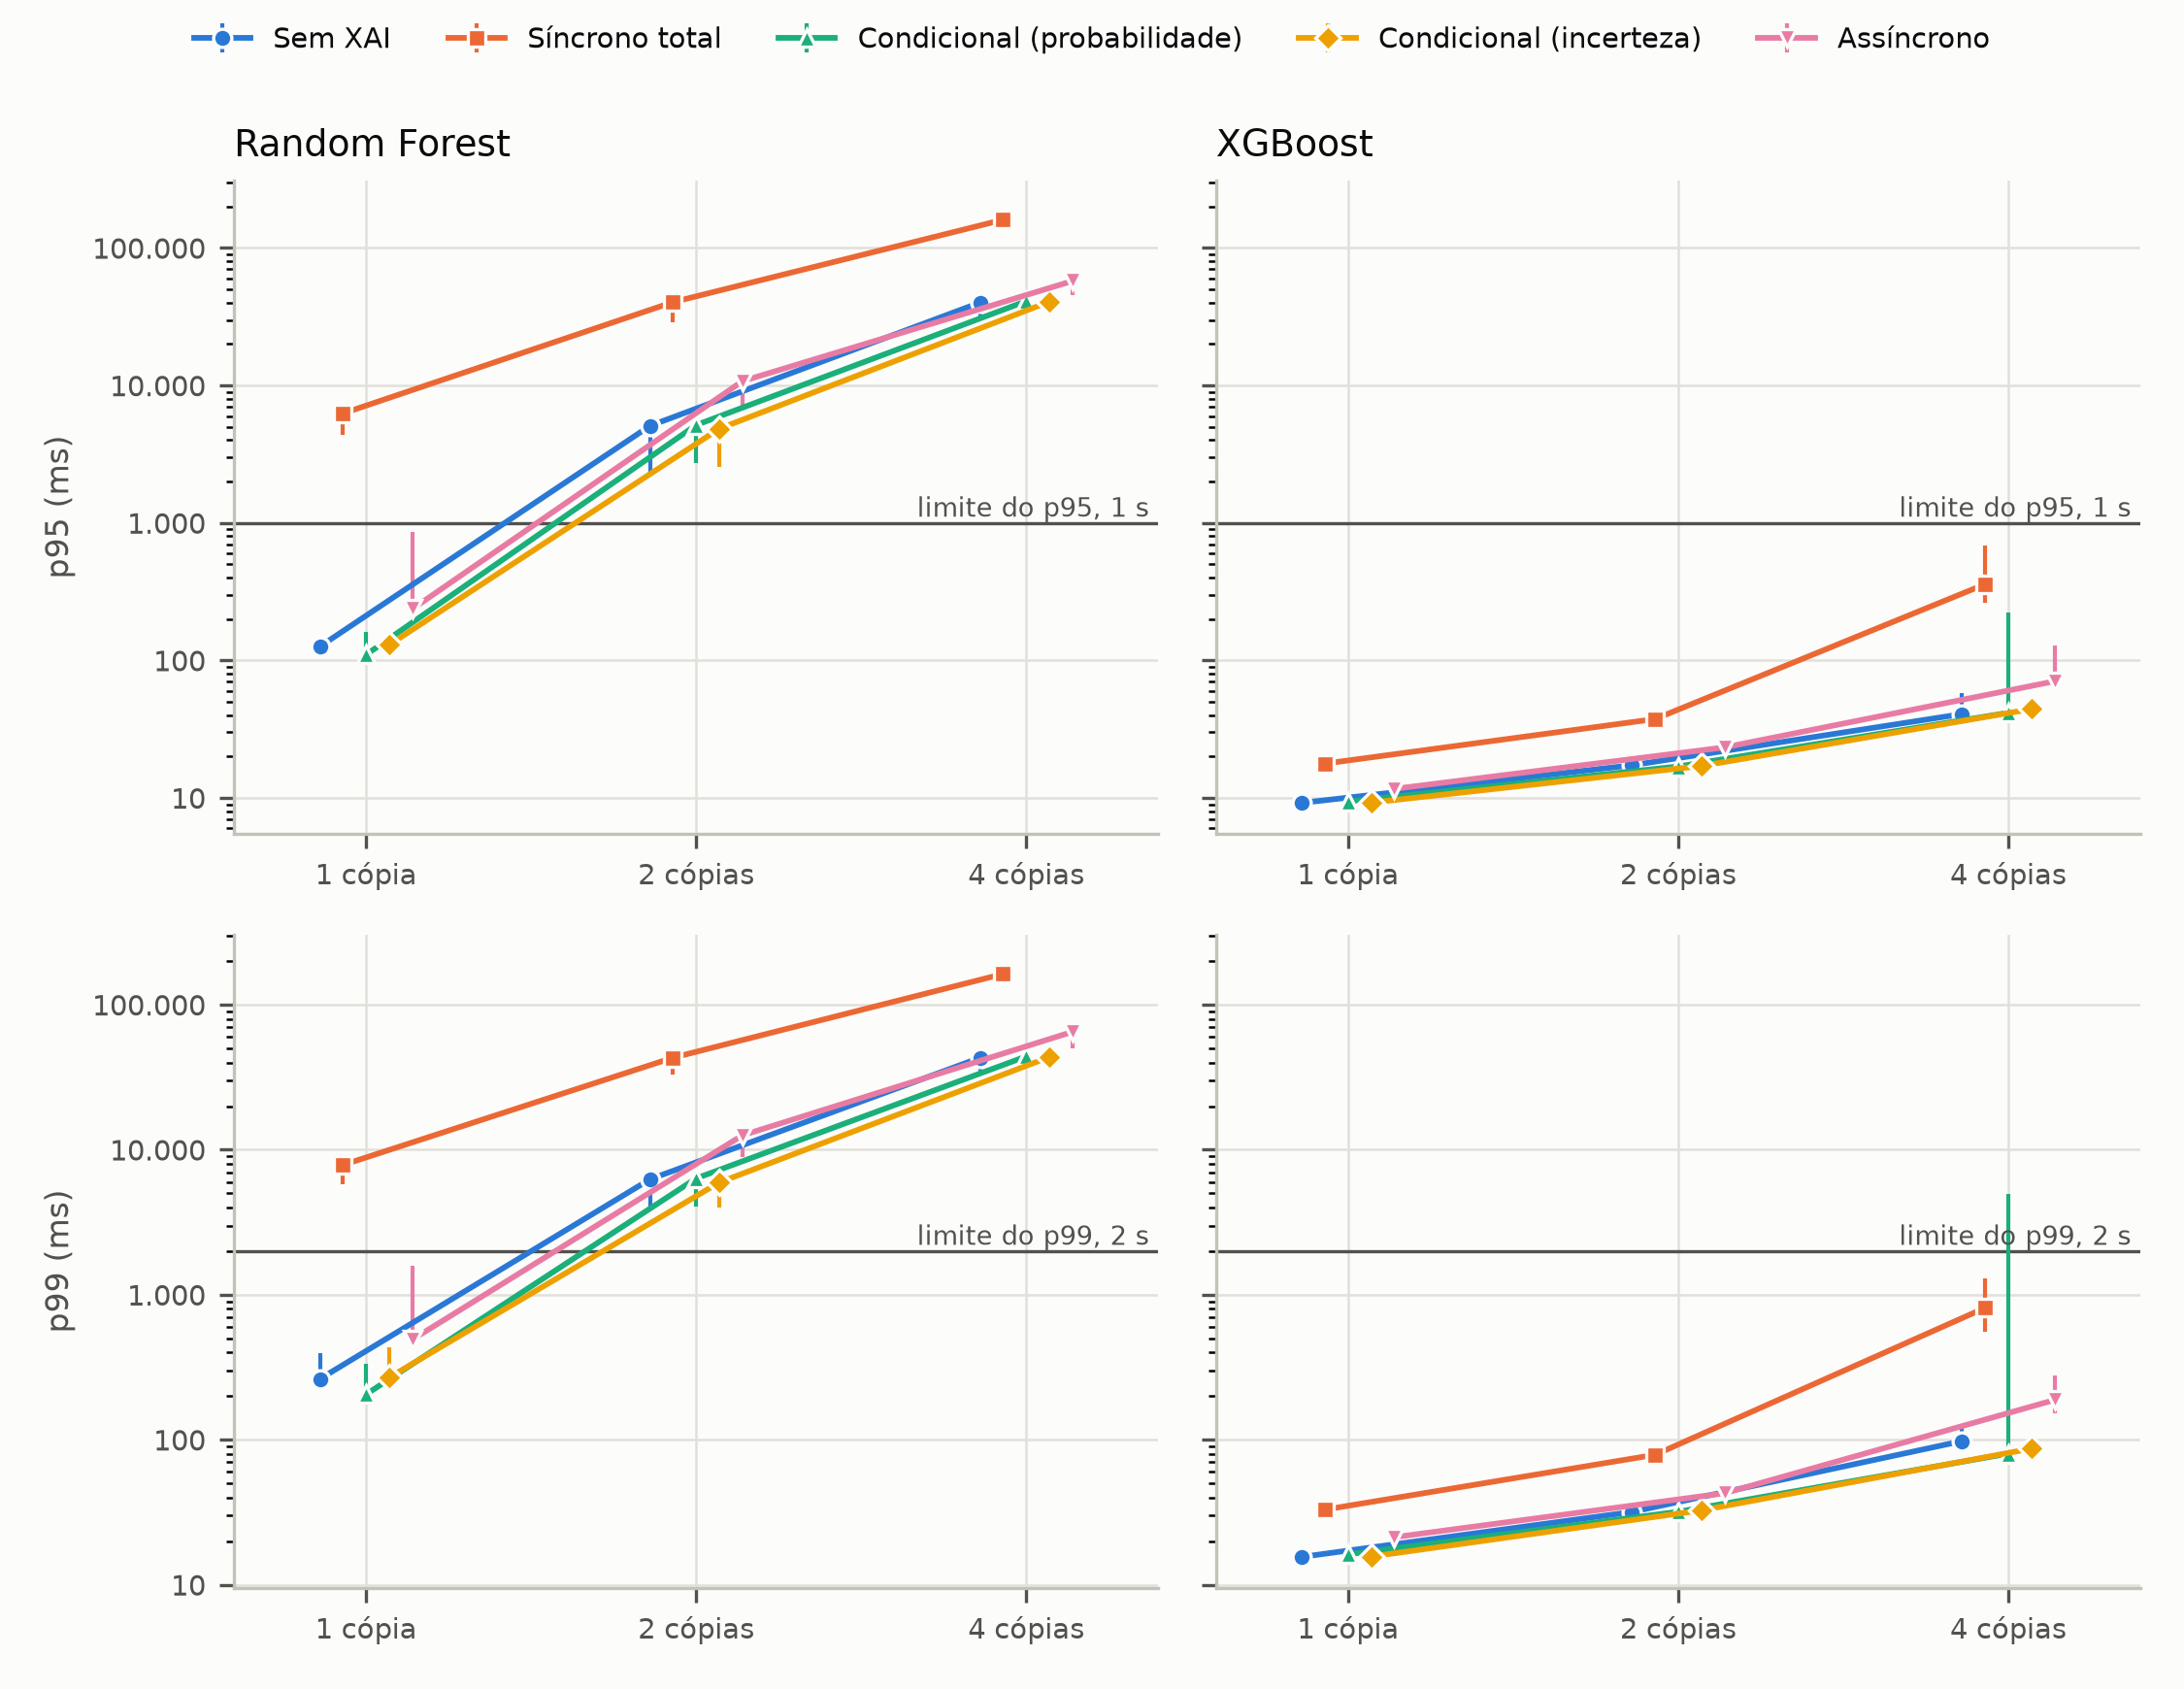
\includegraphics[width=\textwidth]{figuras/latencia-classificacao.png}
  \fonte{Elaborada pelo autor.}
  \nota{Cada ponto é a mediana das 3 execuções, e a barra vai do mínimo ao máximo. As linhas
  horizontais marcam os limites de 1~s no p95 e de 2~s no p99. O eixo vertical é logarítmico.}
\end{figure}

\begin{table}[htbp]
  \centering
  \caption{Mediana do p95 da latência de classificação, em milissegundos}
  \label{tab:latencia}
  \begin{tabular}{llrrr}
    \toprule
    Classificador & Configuração & 1 cópia & 2 cópias & 4 cópias \\
    \midrule
    Random Forest & Sem XAI & 126,2 & 5.086* & 40.103* \\
    & Síncrono total & 6.265* & 40.413* & 160.610* \\
    & Condicional, probabilidade & 110,1 & 5.155* & 41.105* \\
    & Condicional, incerteza & 129,9 & 4.849* & 40.685* \\
    & Assíncrono & 236,6 & 10.751* & 57.541* \\
    \midrule
    XGBoost & Sem XAI & 9,2 & 17,3 & 40,8 \\
    & Síncrono total & 17,8 & 37,5 & 358,7 \\
    & Condicional, probabilidade & 9,4 & 16,9 & 41,6* \\
    & Condicional, incerteza & 9,2 & 17,1 & 44,3 \\
    & Assíncrono & 11,6 & 23,3 & 70,5 \\
    \bottomrule
  \end{tabular}
  \fonte{Elaborada pelo autor.}
  \nota{Mediana das 3 execuções de cada combinação. O asterisco marca as combinações inviáveis.}
\end{table}

A Figura~\ref{fig:pendentes} mostra o maior número de
\termo{fluxo-pendente}{fluxos pendentes de classificação} a cada 10~s, na
\termo{repeticao}{repetição} 1 do Sem XAI, do Síncrono total e do Assíncrono. No XGBoost, o maior
número de fluxos pendentes de uma \termo{execucao}{execução} ficou entre 63 e 865, exceto na
execução que perdeu pacotes, que chegou a 1.241. No Random Forest, o maior número de fluxos
pendentes ficou entre 68 e 727 com 1 cópia, entre 790 e 3.116 com 2 cópias e entre 5.580 e 10.100
com 4 cópias. As três execuções do Síncrono total do Random Forest com 4 cópias
\termo{saturacao}{saturaram}. Nelas, um único intervalo com fluxo pendente cobriu de 99,0\% a
99,7\% do tempo entre o primeiro fluxo emitido e a última classificação.

\begin{figure}[htbp]
  \centering
  \caption{Fluxos pendentes de classificação ao longo da execução}
  \label{fig:pendentes}
  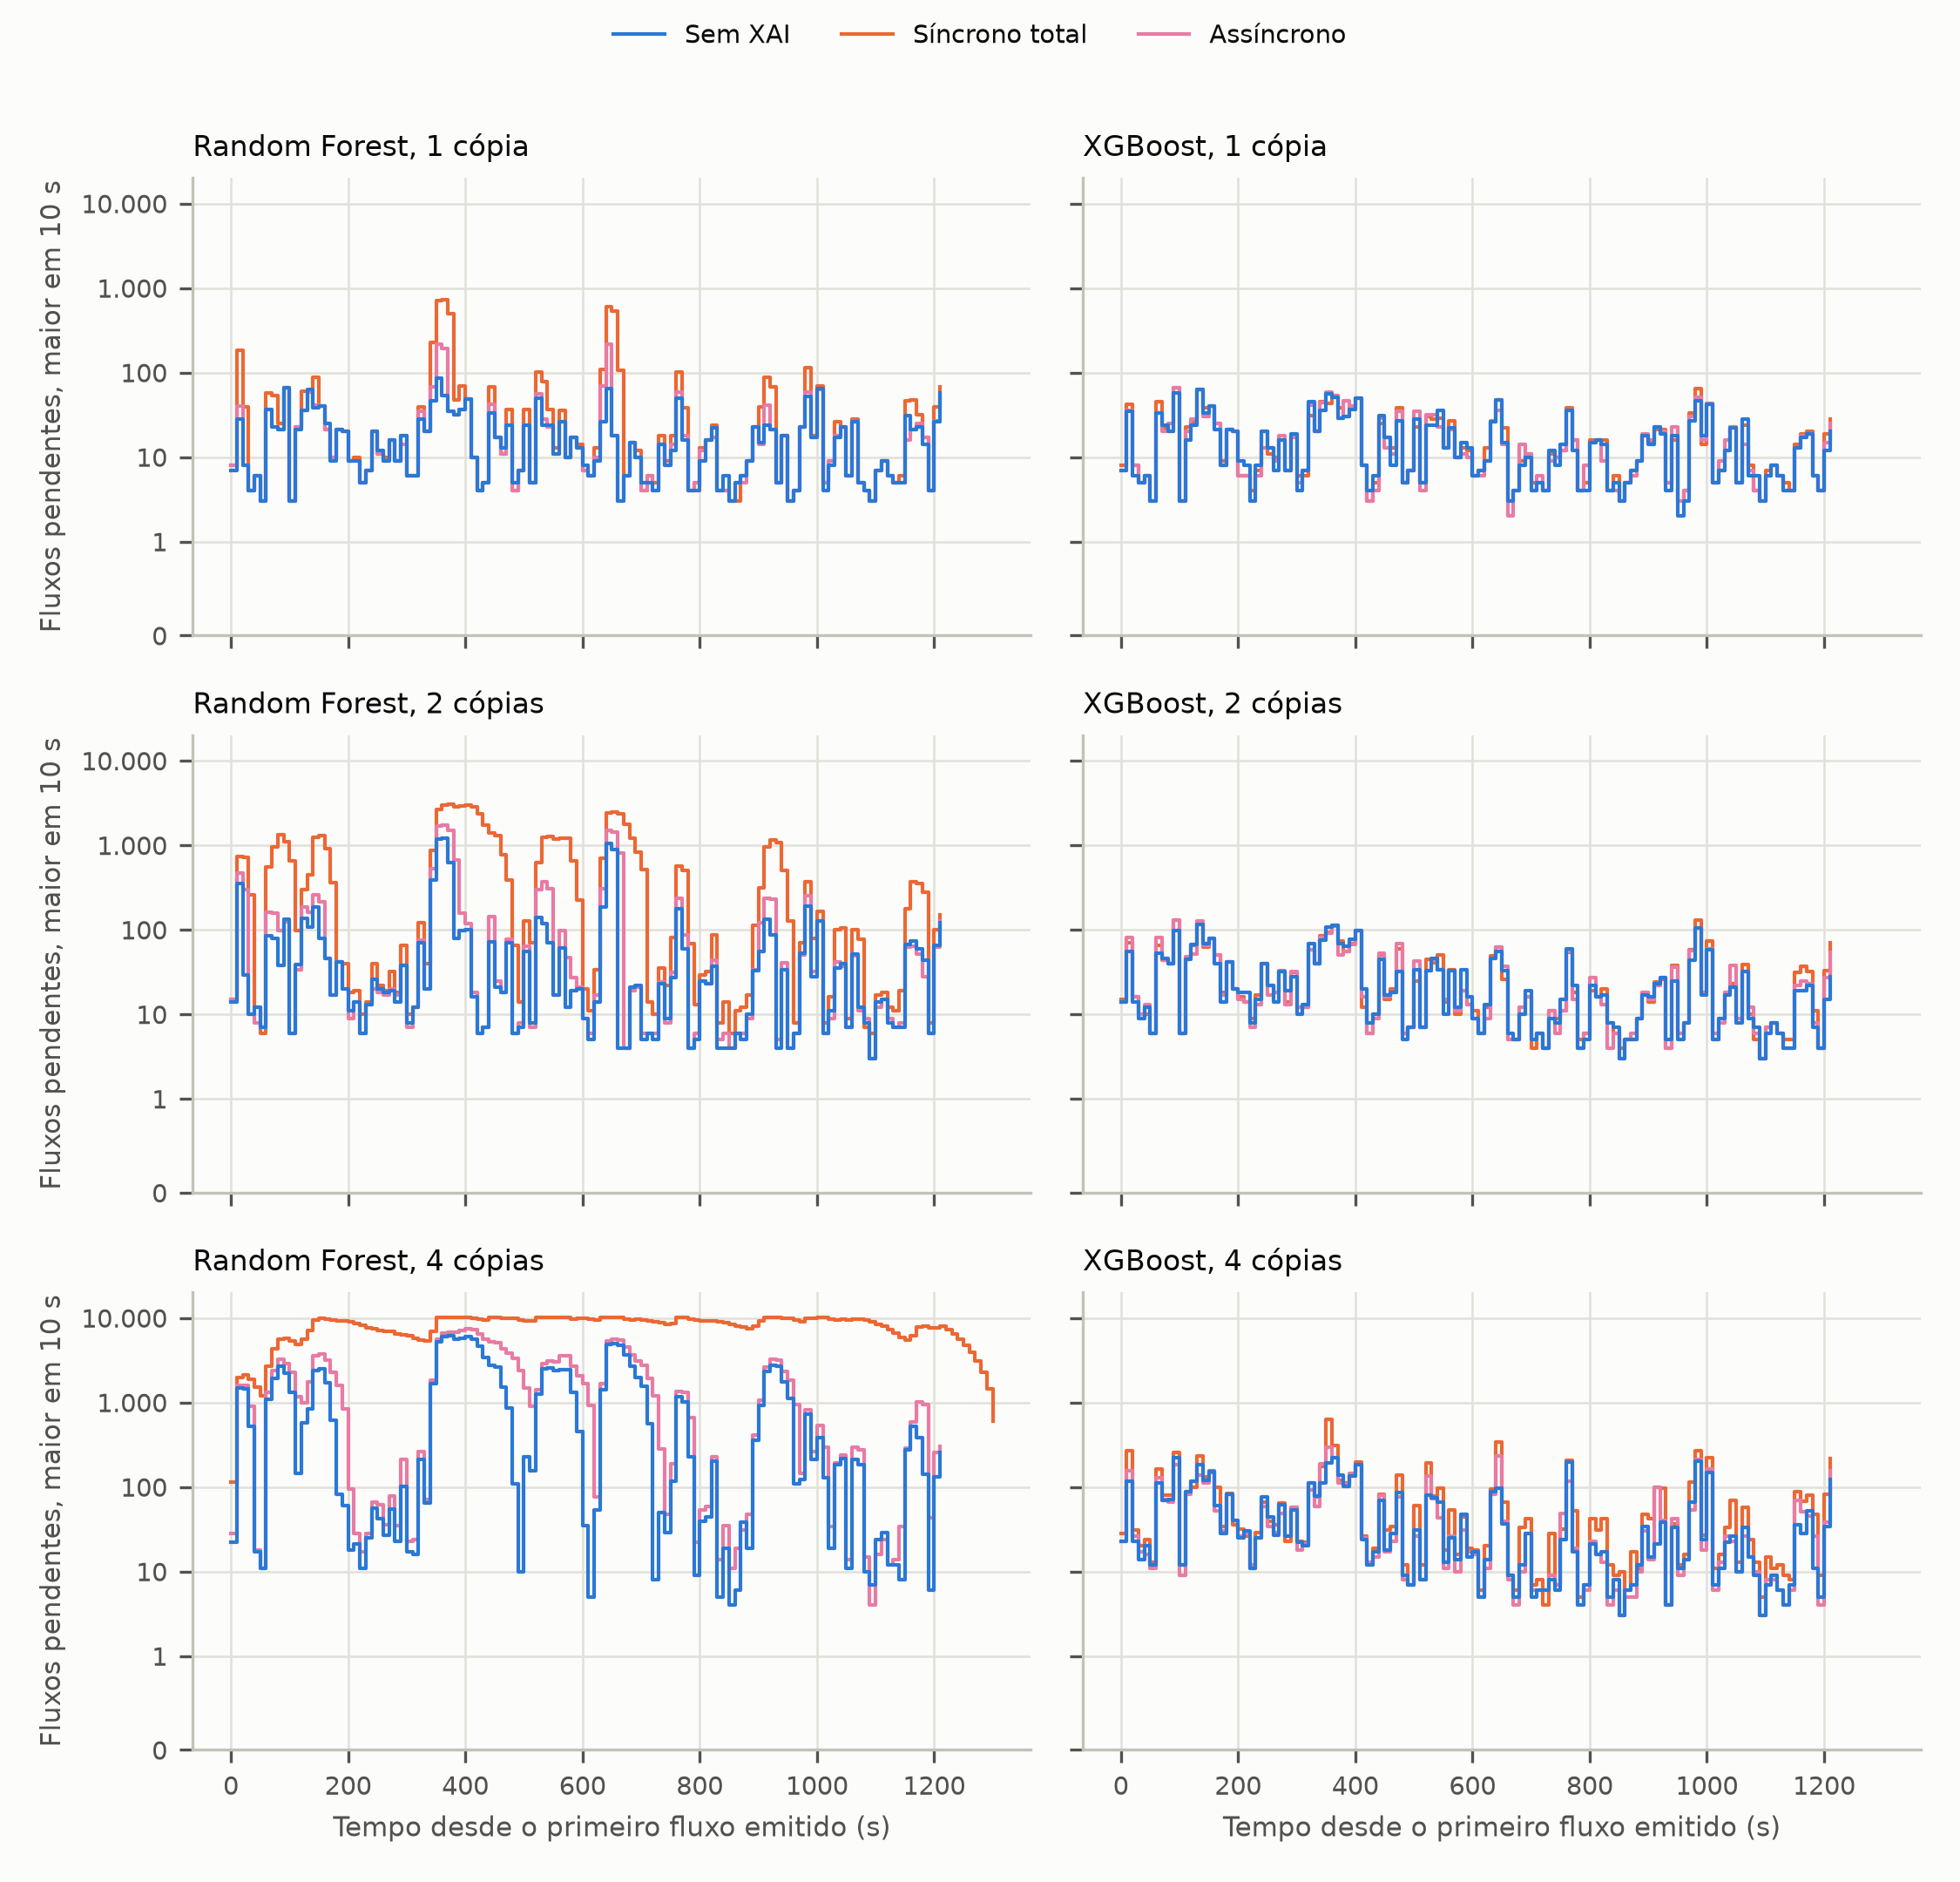
\includegraphics[width=\textwidth]{figuras/pendentes-classificacao.png}
  \fonte{Elaborada pelo autor.}
  \nota{Maior número de fluxos pendentes a cada 10~s, na repetição 1 de cada configuração. O eixo
  vertical é linear entre 0 e 1 e logarítmico acima de 1.}
\end{figure}

\section{Explicações: latência, fila e cobertura}

A Tabela~\ref{tab:explicacoes} traz a mediana do p95 da
\termo{latencia-explicacao}{latência de explicação} e a proporção de \termo{fluxo}{fluxos}
explicados de cada configuração que explica fluxos. Essa proporção é a parte da
\termo{cobertura-explicativa}{cobertura explicativa} que conta os fluxos classificados com a
explicação concluída. No \termo{sincrono-total}{Síncrono total}, a explicação fica disponível junto
com a classificação. Por isso, as duas latências coincidem. Já no \termo{assincrono}{Assíncrono}, a
latência de explicação inclui a espera na \termo{fila-explicacoes}{fila de explicações pendentes}.
No XGBoost, o p95 da latência de explicação ficou menos de 2~ms acima do p95 da
\termo{latencia-classificacao}{latência de classificação}, nas três \termo{carga}{cargas}. No Random
Forest com 1 cópia, porém, o p95 da latência de explicação foi de 1.636~ms, contra 236,6~ms do p95
da latência de classificação.

A Figura~\ref{fig:fila} mostra o tamanho da fila de explicações pendentes nas
\termo{execucao}{execuções} do Assíncrono. No XGBoost, a fila teve no máximo 30
\termo{solicitacao}{solicitações}. No Random Forest, a fila cresceu nos picos de
\termo{emissao}{emissão} de fluxos. O maior tamanho da fila ficou entre 305 e 480 solicitações com
1 cópia e entre 1.869 e 2.085 com 2 cópias. Com 4 cópias, a fila atingiu o limite de 10.000
solicitações. Nessas execuções, o NIDS descartou de 539 a 5.051 solicitações por execução. Em todas
as execuções do Assíncrono, o \termo{processo-explicador}{processo explicador} concluiu as
solicitações aceitas. O \termo{esvaziamento}{tempo de esvaziamento} foi de no máximo 10,0~s, bem
abaixo do limite de 300~s.

\begin{table}[htbp]
  \centering
  \caption{Mediana do p95 da latência de explicação, em milissegundos, e proporção de fluxos explicados}
  \label{tab:explicacoes}
  \setlength{\tabcolsep}{4pt}
  \begin{tabular}{llrrrr}
    \toprule
    Classificador & Configuração & 1 cópia & 2 cópias & 4 cópias & Explicados (\%) \\
    \midrule
    Random Forest & Síncrono total & 6.265 & 40.413 & 160.610 & 100 \\
    & Condicional, probabilidade & 48,5 & 391,2 & 25.812 & 2,8 \\
    & Condicional, incerteza & 59,4 & 324,0 & 42.049 & 0,1 \\
    & Assíncrono & 1.636 & 23.318 & 157.421 & 100* \\
    \midrule
    XGBoost & Síncrono total & 17,8 & 37,5 & 358,7 & 100 \\
    & Condicional, probabilidade & 5,8 & 6,1 & 8,8 & 2,8 \\
    & Condicional, incerteza & 6,4 & 10,8 & 24,1 & 0,1 \\
    & Assíncrono & 13,3 & 24,9 & 72,1 & 100 \\
    \bottomrule
  \end{tabular}
  \fonte{Elaborada pelo autor.}
  \nota{Mediana das 3 execuções de cada combinação. Os explicados são a proporção dos fluxos
  classificados com a explicação concluída. *Com 4 cópias, a mediana foi de 95,9\%.}
\end{table}

\begin{figure}[htbp]
  \centering
  \caption{Fila de explicações pendentes ao longo da execução, no Assíncrono}
  \label{fig:fila}
  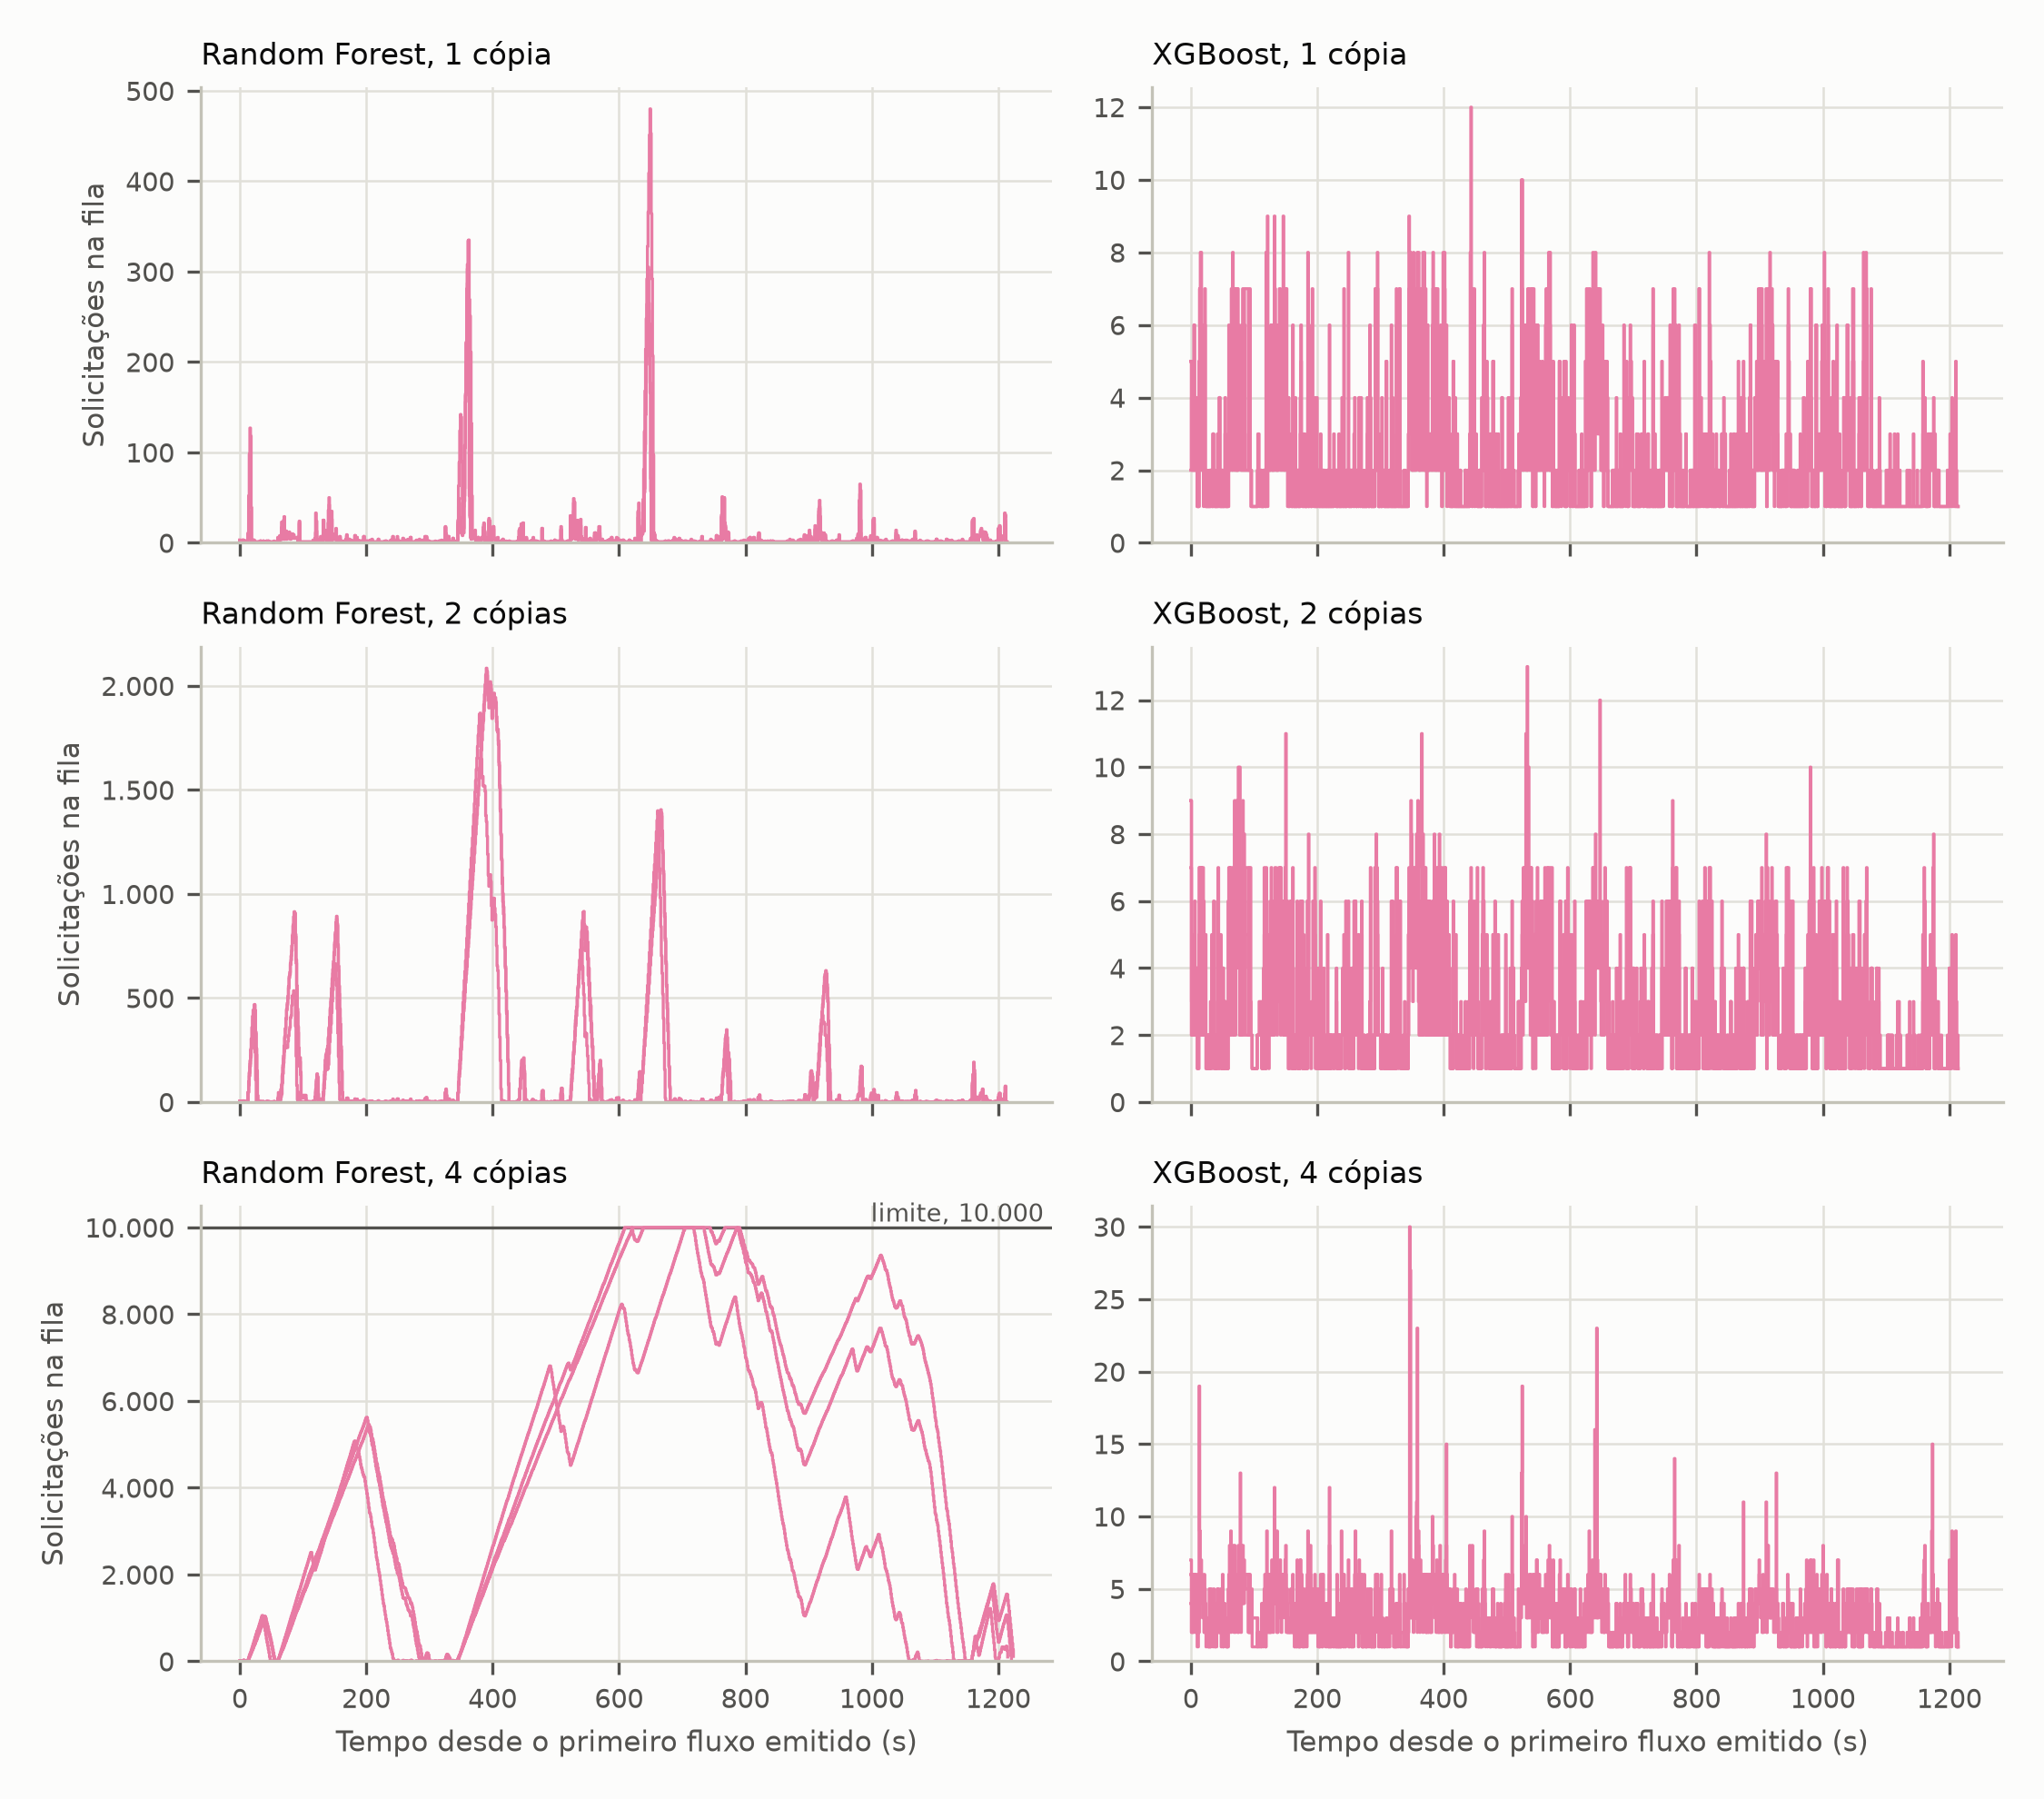
\includegraphics[width=\textwidth]{figuras/fila-explicacoes.png}
  \fonte{Elaborada pelo autor.}
  \nota{Maior tamanho da fila a cada segundo, nas 3 execuções de cada combinação.}
\end{figure}

\section{Uso de recursos}

A Tabela~\ref{tab:cpu} traz o tempo de CPU por \termo{fluxo}{fluxo} classificado do
\termo{processo-classificador}{processo classificador} e do
\termo{processo-explicador}{processo explicador}, com 1 e 4 cópias. O processo classificador é
medido do início ao fim da captura. O processo explicador é medido do fim do carregamento do
classificador ao fim do atendimento das \termo{solicitacao}{solicitações}. Assim, nenhuma das duas
medidas inclui o carregamento do classificador. O tempo de CPU do processo classificador por fluxo
cresceu com a \termo{carga}{carga} em todas as configurações. O crescimento ocorreu até no
\termo{sem-xai}{Sem XAI}, em que o trabalho por fluxo não muda com a carga. No Random Forest, esse
tempo passou de 4,3~ms para 7,1~ms (Seção~\ref{sec:limitacoes}).

O pico de memória residente do processo classificador ficou entre 222 e 386~MiB. O do processo
explicador ficou entre 201 e 204~MiB. Já o pico do extrator cresceu com o número de cópias, de
1.788 a 1.891~MiB com 1 cópia para 4.912 a 4.981~MiB com 4 cópias. O extrator guarda os pacotes de
cada fluxo e mantém cada fluxo emitido até chegar outro pacote com os mesmos endereços, portas e
protocolo, para que o fluxo seguinte da mesma conexão TCP herde o sentido e a duração acumulada. Por
isso, a memória do extrator cresce com o número de fluxos simultâneos. Esse crescimento limita a
carga a 4 cópias (Seção~\ref{sec:matriz}).

\begin{table}[htbp]
  \centering
  \caption{Tempo de CPU por fluxo classificado, em milissegundos}
  \label{tab:cpu}
  \begin{tabular}{llrrrr}
    \toprule
    & & \multicolumn{2}{c}{Processo classificador} & \multicolumn{2}{c}{Processo explicador} \\
    Classificador & Configuração & 1 cópia & 4 cópias & 1 cópia & 4 cópias \\
    \midrule
    Random Forest & Sem XAI & 4,3 & 7,1 & --- & --- \\
    & Síncrono total & 11,7 & 14,8 & --- & --- \\
    & Condicional, probabilidade & 4,2 & 7,3 & --- & --- \\
    & Condicional, incerteza & 4,3 & 7,0 & --- & --- \\
    & Assíncrono & 4,7 & 8,7 & 6,8 & 11,7 \\
    \midrule
    XGBoost & Sem XAI & 0,70 & 0,79 & --- & --- \\
    & Síncrono total & 1,20 & 1,41 & --- & --- \\
    & Condicional, probabilidade & 0,74 & 0,81 & --- & --- \\
    & Condicional, incerteza & 0,70 & 0,86 & --- & --- \\
    & Assíncrono & 0,82 & 0,96 & 0,66 & 0,79 \\
    \bottomrule
  \end{tabular}
  \fonte{Elaborada pelo autor.}
  \nota{Mediana das 3 execuções de cada combinação. O processo explicador só existe no Assíncrono.}
\end{table}

\section{Viabilidade e discussão}
\label{sec:viabilidade}

Pelos critérios de viabilidade da Seção~\ref{sec:matriz}, 18 das 30 combinações de
\termo{classificador}{classificador}, \termo{configuracao}{configuração de explicação} e \termo{nivel-carga}{nível de
carga} foram viáveis. No XGBoost, as cinco configurações foram viáveis com 1, 2 e 4 cópias, exceto o
\termo{sincrono-condicional}{Síncrono condicional} pelo critério de probabilidade com 4 cópias. Essa
combinação foi viável em 2 das 3 \termo{execucao}{execuções}, e uma combinação só é viável quando as
suas 3 execuções são viáveis. No Random Forest, só houve combinações viáveis com 1 cópia, no
\termo{sem-xai}{Sem XAI}, nos dois critérios do Síncrono condicional e no
\termo{assincrono}{Assíncrono}. O \termo{sincrono-total}{Síncrono total} do Random Forest não foi
viável em nenhum nível de carga.

Os resultados sustentam a primeira parte da hipótese, segundo a qual a explicação acrescenta um
custo que varia com a estratégia de explicação e com a \termo{carga}{carga}. A
\termo{sobrecarga}{sobrecarga de latência} cresceu com a carga no Síncrono total e no Assíncrono, nos
dois classificadores. No p95 do XGBoost, a sobrecarga do Síncrono total foi de 8,6, 20 e 318~ms com
1, 2 e 4 cópias. No Assíncrono, ela foi de 2,4, 6,0 e 30~ms. No Random Forest com 1 cópia, o
Síncrono total acrescentou 6,1~s ao p95, e o Assíncrono, 110~ms. Essas sobrecargas atendem à regra
de diferença da Seção~\ref{sec:matriz}.

Os resultados também sustentam a segunda parte da hipótese, segundo a qual explicar só alguns
\termo{fluxo}{fluxos}, ou explicar fora do caminho da classificação, reduz esse custo. Com o
Síncrono condicional, a \termo{latencia-classificacao}{latência de classificação} não se distinguiu
da do Sem XAI pela regra da Seção~\ref{sec:matriz}. Em troca, o critério de probabilidade explicou
2,8\% dos fluxos classificados, e o de incerteza, cerca de 0,1\%. Como o
critério de probabilidade explica os fluxos classificados como ataque, a
\termo{cobertura-explicativa}{cobertura explicativa} desse critério acompanha a proporção de fluxos
de ataque do trecho, de cerca de 2,8\%. Tolay (2026) observa essa dependência no CICIoT2023. Na
medição desse autor, uma política que explica todos os ataques previstos e parte dos benignos
economizou de 15\% a 23\% do trabalho de explicação num conjunto de teste balanceado e de 1,7\% a
2,6\% no conjunto com a distribuição original, dominada por ataques. Num tráfego com mais ataques,
portanto, o custo do critério de probabilidade se aproximaria do custo do Síncrono total. A campanha
não mediu essa condição.

O Assíncrono tirou a explicação do \termo{caminho}{caminho da classificação} e explicou todos os
fluxos enquanto a \termo{fila-explicacoes}{fila de explicações pendentes} teve vaga
(Tabela~\ref{tab:explicacoes} e Figura~\ref{fig:fila}). O custo passou para a \termo{latencia-explicacao}{latência de
explicação} e para o \termo{processo-explicador}{processo explicador}. Mesmo sem esperar a
explicação, porém, o Assíncrono elevou a latência de classificação. No Random Forest com 1 cópia, o
p95 passou de 126~ms para 237~ms. Quase toda essa diferença ocorreu antes de $t_1$, na espera dos
fluxos pelo \termo{processo-classificador}{processo classificador}. Essa espera cresceu porque a média do
\termo{tempo-inferencia}{tempo de inferência} passou de 3,9~ms para 4,2~ms. Como o processo
explicador roda em outro núcleo de desempenho, esse aumento não vem da divisão do núcleo do
processo classificador. O experimento não mede a causa. Uma explicação possível é a disputa dos
recursos que os núcleos compartilham, como a memória cache de último nível. O tempo de CPU mostra,
além disso, que o Assíncrono não reduz o trabalho de explicar (Tabela~\ref{tab:cpu}). No Random
Forest com 1 cópia, ele dividiu o custo entre 4,7~ms no processo classificador e 6,8~ms no processo
explicador por fluxo, contra 11,7~ms no processo classificador do Síncrono total. O Assíncrono,
portanto, leva esse trabalho para outro núcleo, que precisa estar livre.

No Random Forest, a classificação sozinha já passou do limite de latência com 2 cópias, mas não pela
carga média. A carga média dessas execuções, de 40,7 fluxos por segundo, com 4,7~ms por inferência,
ocupou o processo classificador por cerca de 19\% do tempo. Os \termo{fluxo-pendente}{fluxos pendentes} se acumularam
nos picos de \termo{emissao}{emissão}, em que o extrator chegou a emitir 508 fluxos num segundo, e o
acúmulo se desfez entre os picos. Só o Síncrono total com 4 cópias \termo{saturacao}{saturou} o NIDS
(Figura~\ref{fig:pendentes}).

A diferença entre os dois classificadores aparece também na medição de Tolay (2026), feita fora de
um NIDS, no CICIoT2023. Com lotes de 1 registro, o TreeSHAP levou 0,126~s no Random Forest e
0,0033~s no XGBoost. Como os classificadores e o processador diferem dos deste trabalho, os valores
absolutos não se comparam. Nos dois trabalhos, porém, explicar o Random Forest custa muito mais que
explicar o XGBoost. Este trabalho acrescenta o efeito desse custo na entrega da classificação sob
carga.

Nugraha, Jnanashree e Bauschert (2025) medem de 0,02~s a 0,08~s por explicação do TreeSHAP num
detector XGBoost, fora de um sistema que recebe tráfego, e concluem que detecção precisa e
interpretabilidade quase em tempo real podem coexistir. Os resultados do XGBoost neste trabalho são
compatíveis com essa conclusão, agora com a latência medida na entrega da classificação. Le et al.
(2026) avaliam, numa simulação com custos de explicação normalizados e sem medir latências num NIDS,
políticas que escolhem entre
suprimir, adiar ou gerar a explicação local completa. A fila de explicações pendentes do Assíncrono
do Random Forest é o tipo de acúmulo que essas políticas procuram controlar, e as medições deste
trabalho fornecem os custos que elas tratam como parâmetros.

\section{Limitações}
\label{sec:limitacoes}

Os resultados valem para as condições do experimento e não implicam equivalência com redes físicas
de produção nem garantia de tempo real estrito. Cinco condições limitam o alcance dos resultados.
\begin{itemize}
  \item \textbf{Máquina única}: a rede é emulada numa única máquina, que também reproduz o tráfego.
  \item \textbf{Implementação do processo classificador}: o
  \termo{processo-classificador}{processo classificador} roda em Python, com uma \emph{thread}.
  \item \textbf{Trecho de tráfego}: o tráfego é um trecho de 20 minutos de um único dia, cujos
  ataques são todos de FTP-Patator. Por isso, o \termo{sincrono-condicional}{Síncrono condicional}
  pelo critério de probabilidade explica uma pequena parte dos \termo{fluxo}{fluxos}.
  \item \textbf{Cópias simultâneas}: como as cópias do trecho começam juntas, os picos de emissão das
  cópias coincidem. Por isso, os picos de \termo{carga}{carga} crescem na mesma proporção do número
  de cópias. Com picos de emissão desencontrados, a mesma carga média teria picos menores. O Random
  Forest, que passou do limite de latência pelo acúmulo de fluxos nos picos de emissão, poderia então
  atender cargas maiores. A campanha não mediu esse caso.
  \item \textbf{Fluxos sem correspondência}: os fluxos das conexões anteriores ao início do trecho não
  correspondem aos fluxos rotulados do dataset, embora façam parte da carga.
\end{itemize}
Além disso, as latências medidas começam no fim da extração dos atributos e não incluem a espera até
a \termo{emissao}{emissão do fluxo}, que pode chegar a 120~s.

O \termo{tempo-inferencia}{tempo de inferência} cresceu com a carga. No \termo{sem-xai}{Sem XAI}
do Random Forest, que não inclui nenhuma espera, a média subiu de 3,9~ms com 1 cópia para 6,4~ms
com 4 cópias. A frequência do núcleo do processo classificador, lida a cada segundo, também subiu
com a carga. Como uma frequência mais alta encurtaria a inferência, a frequência lida não explica
esse aumento. A leitura de cada segundo, porém, não mostra a frequência durante cada inferência. Os
núcleos lógicos que dividem os núcleos físicos do processo classificador e do
\termo{processo-explicador}{processo explicador} não recebem processo do experimento
(Seção~\ref{sec:ambiente}). Mesmo assim, chegaram a 51\% a 100\% de ocupação em algum segundo de
cada \termo{execucao}{execução}. O experimento não separa as causas do aumento do tempo de
inferência, como a disputa dos núcleos físicos e da memória com outros processos. Parte da
\termo{sobrecarga}{sobrecarga de latência} medida nas cargas maiores vem, assim, da máquina, e não
só do NIDS.

Cinco regras de análise foram fixadas depois da campanha, com os resultados já medidos
(Seção~\ref{sec:matriz}). Os limites de latência e de \termo{descarte}{descartes}, ao contrário,
foram fixados no \termo{piloto}{piloto}, antes da campanha. Só duas conclusões mudariam com outras
regras. O Síncrono condicional do XGBoost pelo critério de
probabilidade com 4 cópias seria viável se bastassem 2 das 3 execuções. A
\termo{repeticao}{repetição} 3 do \termo{assincrono}{Assíncrono} do XGBoost com 4 cópias seria
inviável se uma regra reprovasse a \termo{fila-explicacoes}{fila de explicações pendentes} que
volta, no último décimo da execução, ao maior tamanho que já tinha atingido.

Com 3 execuções por combinação, o critério de diferença entre combinações é descritivo e não dá
uma probabilidade de erro (Seção~\ref{sec:matriz}). A execução do XGBoost que perdeu 0,07\% dos
pacotes na captura, e por isso teve 1,2\% dos fluxos com atributos diferentes dos da leitura do
arquivo, continua na análise, porque a perda de pacotes não invalida uma execução.

\chapter{Considerações finais}
\label{cap:conclusao}

Este trabalho perguntou se é viável gerar explicações TreeSHAP das classificações durante a
operação de um NIDS baseado em aprendizado de máquina, sem que a
\termo{latencia-classificacao}{latência de classificação} ultrapasse os limites do experimento. Nas
condições do experimento, a resposta depende do \termo{classificador}{classificador}. Com o XGBoost,
explicar foi viável em todas as \termo{configuracao}{configurações de explicação} até 4 cópias do trecho, inclusive
explicando todos os \termo{fluxo}{fluxos} antes de entregar a classificação. A única exceção foi o
\termo{sincrono-condicional}{Síncrono condicional} pelo critério de probabilidade com 4 cópias, em
que uma \termo{execucao}{execução} perdeu pacotes na captura. Com o Random Forest, explicar todos os
fluxos só foi viável no \termo{assincrono}{Assíncrono}, que tira a explicação do
\termo{caminho}{caminho da classificação}. Mesmo no Assíncrono, explicar todos os fluxos só foi
viável com 1 cópia, o único \termo{nivel-carga}{nível de carga} em que o \termo{sem-xai}{Sem XAI} do
Random Forest foi viável.

Cada estratégia de explicação paga um custo diferente pela explicação. O
\termo{sincrono-total}{Síncrono total} explica todos os fluxos e soma o tempo da explicação à
latência de classificação. Por isso, o Síncrono total do Random Forest foi inviável já com 1 cópia.
O Síncrono condicional teve latência de classificação que não se distinguiu da do Sem XAI. Em
troca, explicou 2,8\% dos fluxos pelo critério de probabilidade e cerca de 0,1\% pelo critério de
incerteza. A proporção explicada pelo critério de probabilidade acompanha a proporção de ataques do
tráfego. O Assíncrono teve \termo{sobrecarga}{sobrecarga de latência} menor que a do Síncrono total
e explicou todos os fluxos enquanto a \termo{fila-explicacoes}{fila de explicações pendentes} teve
vaga. Em troca, atrasou as explicações e ocupou outro núcleo. No Random Forest com 4 cópias, o NIDS
descartou \termo{solicitacao}{solicitações de explicação} porque a fila encheu.

Os resultados valem para uma única máquina, um trecho de 20 minutos de um único dia e cópias com
picos de emissão coincidentes (Seção~\ref{sec:limitacoes}).

\section{Contribuições}

O trabalho mede as quatro \termo{estrategia}{estratégias de explicação} num mesmo NIDS, com o mesmo
\termo{caminho}{caminho da classificação}, com dois \termo{classificador}{classificadores} e três
\termo{nivel-carga}{níveis de carga}. As medidas são a
\termo{latencia-classificacao}{latência de classificação}, a
\termo{latencia-explicacao}{latência de explicação}, o uso de recursos e a
\termo{cobertura-explicativa}{cobertura explicativa}. O trabalho também contribui com um ambiente em
que a \termo{carga}{carga} cresce sem alterar os atributos dos \termo{fluxo}{fluxos}, porque cada
fluxo de uma cópia do trecho tem os mesmos atributos do fluxo correspondente do trecho. O código, as
configurações, as decisões do delineamento experimental e o guia de reprodução estão no repositório
do trabalho (Seção~\ref{sec:disponibilidade}).
Seguido numa cópia nova do repositório, o guia de reprodução gerou conjuntos de treino, validação e
teste, \termo{modelo-congelado}{modelos congelados}, trechos de PCAP e classificações e explicações
das leituras por arquivo idênticos aos do experimento.

Parte das dificuldades do trabalho veio das ferramentas e dos dados. O \texttt{tcpreplay} 4.5.2,
distribuído pelo Ubuntu 26.04, não enviava os quadros acima de 4.064 bytes quando a MTU passava de
uma página de memória. Por isso, a reprodução usou a versão 4.6.2, compilada a partir do
código-fonte. Os dois comprimentos de cabeçalho do Improved CIC-IDS2017 foram gravados em inteiros
de 16 bits e diferem do que o extrator calcula em operação. Por isso, esses dois atributos ficaram
fora das entradas do classificador (Seção~\ref{sec:dados}). Na campanha, uma
\termo{execucao}{execução} perdeu pacotes na captura. Por isso, a auditoria passou a registrar a
reprovação da validação dessa execução como explicada pela perda (Seção~\ref{sec:limitacoes}).

\section{Trabalhos futuros}

As limitações da Seção~\ref{sec:limitacoes} indicam os trabalhos futuros.
\begin{itemize}
  \item Medir as estratégias com cópias de picos de emissão desencontrados, para verificar se o
  Random Forest atende cargas maiores quando os picos não coincidem.
  \item Medir as estratégias com tráfego de outros dias, com outros ataques, que mudam a
  \termo{cobertura-explicativa}{cobertura explicativa} do critério de probabilidade.
  \item Separar as causas do aumento do \termo{tempo-inferencia}{tempo de inferência} com a
  \termo{carga}{carga}, mantendo fixa a frequência dos núcleos.
  \item Avaliar políticas que escolhem a ação de explicação conforme o tamanho da
  \termo{fila-explicacoes}{fila de explicações pendentes}, como as de Le et al. (2026), com os custos
  medidos neste trabalho.
\end{itemize}

% ---------------------------------------------------------------------------
% Elementos pós-textuais
% ---------------------------------------------------------------------------
\postextual

% Referências manuais, em ordem alfabética, só com as fontes citadas.
\chapter*{Referências}
\phantomsection
\addcontentsline{toc}{chapter}{\texorpdfstring{\MakeTextUppercase{Referências}}{Referências}}
\begingroup
\SingleSpacing
\setlength{\parindent}{0pt}
\setlength{\parskip}{\baselineskip}
\raggedright
ADADI, Amina; BERRADA, Mohammed. Peeking inside the black-box: a survey on explainable artificial
intelligence (XAI). \textbf{IEEE Access}, [\emph{s. l.}], v. 6, p. 52138--52160, 2018. DOI:
10.1109/ACCESS.2018.2870052.\par

APPNETA. \textbf{Tcpreplay}. Versão 4.6.2. [\emph{S. l.}]: GitHub, 2026. Disponível em:
\url{https://github.com/appneta/tcpreplay}. Acesso em: 17 nov. 2026.\par

BERTOLI, Gustavo de Carvalho \emph{et al.} Abordagem fim-a-fim para uso de aprendizado de máquina
em IDS: caso de detecção \emph{stateless} para TCP Scan. \emph{In}: SIMPÓSIO BRASILEIRO DE
SEGURANÇA DA INFORMAÇÃO E DE SISTEMAS COMPUTACIONAIS, 20., 2020, Petrópolis. \textbf{Anais}
[\ldots]. Porto Alegre: Sociedade Brasileira de Computação, 2020. p. 271--284. DOI: 10.5753/sbseg.2020.19243.\par

BREIMAN, Leo. Random forests. \textbf{Machine Learning}, [\emph{s. l.}], v. 45, n. 1, p. 5--32,
2001. DOI: 10.1023/A:1010933404324.\par

CHEN, Tianqi; GUESTRIN, Carlos. XGBoost: a scalable tree boosting system. \emph{In}: ACM SIGKDD
INTERNATIONAL CONFERENCE ON KNOWLEDGE DISCOVERY AND DATA MINING, 22., 2016, San Francisco.
\textbf{Proceedings} [\ldots]. New York: ACM, 2016. p. 785--794. DOI: 10.1145/2939672.2939785.\par

DASH, Sandhyarani; ACKEN, John M. Intrusion detection latency: the neglected metric.
\textbf{Cybersecurity}, [\emph{s. l.}], v. 9, n. 1, art. 144, 2026. DOI:
10.1186/s42400-026-00574-7.\par

ENGELEN, Gints. \textbf{CICFlowMeter}. Commit 13a061520b. [\emph{S. l.}]: GitHub, 2022. Disponível
em: \url{https://github.com/GintsEngelen/CICFlowMeter}. Acesso em: 17 nov. 2026.\par

ENGELEN, Gints. \textbf{CNS2022\_Code}. [\emph{S. l.}]: GitHub, 2023. Disponível em:
\url{https://github.com/GintsEngelen/CNS2022_Code}. Acesso em: 17 nov. 2026.\par

ENGELEN, Gints; RIMMER, Vera; JOOSEN, Wouter. Troubleshooting an intrusion detection dataset: the
CICIDS2017 case study. \emph{In}: IEEE SECURITY AND PRIVACY WORKSHOPS, 2021, San Francisco.
\textbf{Proceedings} [\ldots]. [\emph{S. l.}]: IEEE, 2021. p. 7--12. DOI:
10.1109/SPW53761.2021.00009.\par

FAWCETT, Tom. An introduction to ROC analysis. \textbf{Pattern Recognition Letters}, [\emph{s. l.}],
v. 27, n. 8, p. 861--874, 2006. DOI: 10.1016/j.patrec.2005.10.010.\par

HENDRICKX, Kilian \emph{et al.} Machine learning with a reject option: a survey. \textbf{Machine
Learning}, [\emph{s. l.}], v. 113, p. 3073--3110, maio 2024. DOI: 10.1007/s10994-024-06534-x.\par

LANTZ, Bob; HELLER, Brandon; MCKEOWN, Nick. A network in a laptop: rapid prototyping for
software-defined networks. \emph{In}: ACM SIGCOMM WORKSHOP ON HOT TOPICS IN NETWORKS, 9., 2010,
Monterey. \textbf{Proceedings} [\ldots]. New York: ACM, 2010. p. 1--6. DOI:
10.1145/1868447.1868466.\par

LE, Tran Duc \emph{et al.} Explanation-surface governance in
XAI-enabled network intrusion detection under resource constraints. \textbf{Research Square},
2026. Preprint, versão 1. DOI: 10.21203/rs.3.rs-9800570/v1.\par

LIU, Lisa \emph{et al.} Error prevalence in NIDS
datasets: a case study on CIC-IDS-2017 and CSE-CIC-IDS-2018. \emph{In}: IEEE CONFERENCE ON
COMMUNICATIONS AND NETWORK SECURITY, 2022, Austin. \textbf{Proceedings} [\ldots]. [\emph{S. l.}]:
IEEE, 2022. p. 254--262. DOI: 10.1109/CNS56114.2022.9947235.\par

LUNDBERG, Scott M.; LEE, Su-In. A unified approach to interpreting model predictions. \emph{In}:
CONFERENCE ON NEURAL INFORMATION PROCESSING SYSTEMS, 31., 2017, Long Beach. \textbf{Advances in
Neural Information Processing Systems 30}. Red Hook: Curran Associates, 2017. p. 4765--4774.\par

LUNDBERG, Scott M. \emph{et al.} From local explanations to global understanding with explainable
AI for trees. \textbf{Nature Machine Intelligence}, [\emph{s. l.}], v. 2, n. 1, p. 56--67, 2020.
DOI: 10.1038/s42256-019-0138-9.\par

NUGRAHA, Beny; JNANASHREE, Abhishek Venkatesh; BAUSCHERT, Thomas. A versatile XAI-based framework
for efficient and explainable intrusion detection systems. \textbf{Annals of Telecommunications},
[\emph{s. l.}], v. 80, n. 11-12, p. 1095--1120, 2025. DOI: 10.1007/s12243-025-01118-9.\par

OGUNSEYI, Taiwo Blessing \emph{et al.} Performance analysis of explainable deep learning-based
intrusion detection systems for IoT networks: a systematic review. \textbf{Sensors},
[\emph{s. l.}], v. 26, n. 2, art. 363, 2026. DOI: 10.3390/s26020363.\par

SCIKIT-LEARN DEVELOPERS. \textbf{Ensemble methods}. Versão 1.9.1. [\emph{S. l.}]: scikit-learn,
[2026]. Disponível em: \url{https://scikit-learn.org/stable/modules/ensemble.html}. Acesso em: 21
nov. 2026.\par

SHAP. \textbf{shap}. Versão 0.54.1. [\emph{S. l.}]: GitHub, 2026. Disponível em:
\url{https://github.com/shap/shap}. Acesso em: 17 nov. 2026.\par

SHAPLEY, Lloyd S. A value for n-person games. \emph{In}: KUHN, Harold W.; TUCKER, Albert W. (ed.).
\textbf{Contributions to the theory of games}. Princeton: Princeton University Press, 1953. v. 2,
p. 307--318. DOI: 10.1515/9781400881970-018.\par

SHARAFALDIN, Iman; HABIBI LASHKARI, Arash; GHORBANI, Ali A. Toward generating a new intrusion
detection dataset and intrusion traffic characterization. \emph{In}: INTERNATIONAL CONFERENCE ON
INFORMATION SYSTEMS SECURITY AND PRIVACY, 4., 2018, Funchal. \textbf{Proceedings} [\ldots].
[\emph{S. l.}]: SciTePress, 2018. p. 108--116. DOI: 10.5220/0006639801080116.\par

SHWARTZ-ZIV, Ravid; ARMON, Amitai. Tabular data: deep learning is not all you need.
\textbf{Information Fusion}, [\emph{s. l.}], v. 81, p. 84--90, 2022. DOI:
10.1016/j.inffus.2021.11.011.\par

THE KERNEL DEVELOPMENT COMMUNITY. \textbf{Segmentation offloads}. Versão 7.4.0-rc3. [\emph{S. l.}]:
The Linux Kernel Documentation, [2026]. Disponível em:
\url{https://docs.kernel.org/networking/segmentation-offloads.html}. Acesso em: 19 nov. 2026.\par

TOLAY, Abdurrahman. Beyond detection accuracy: measuring explanation cost, stability, and utility
for resource-aware IoT intrusion detection. \textbf{arXiv}, 2026. Preprint 2608.10349v1. DOI:
10.48550/arXiv.2608.10349. Disponível em: \url{https://arxiv.org/abs/2608.10349}. Acesso em: 17
nov. 2026.\par

XGBOOST DEVELOPERS. \textbf{XGBoost parameters}. [\emph{S. l.}]: XGBoost, [2026]. Disponível em:
\url{https://xgboost.readthedocs.io/en/stable/parameter.html}. Acesso em: 21 nov. 2026.\par

ZUECH, Richard; KHOSHGOFTAAR, Taghi M.; WALD, Randall. Intrusion detection and big heterogeneous
data: a survey. \textbf{Journal of Big Data}, [\emph{s. l.}], v. 2, n. 1, art. 3, 2015. DOI:
10.1186/s40537-015-0013-4.\par
\endgroup

\chapter*{Glossário}
\phantomsection
\addcontentsline{toc}{chapter}{\texorpdfstring{\MakeTextUppercase{Glossário}}{Glossário}}
\begin{description}
  \item[Assíncrono]\phantomsection\label{gl:assincrono} Estratégia de explicação em que a classificação fica disponível sem esperar pela explicação. O processo explicador gera a explicação depois da entrega da classificação.
  \item[Caminho da classificação]\phantomsection\label{gl:caminho} Etapas de um fluxo entre o fim da extração de atributos ($t_0$) e a entrega da classificação ($t_3$). Uma explicação está no caminho da classificação quando a entrega espera por ela.
  \item[Campanha experimental]\phantomsection\label{gl:campanha} Conjunto de execuções, com suas repetições, que cobre todas as combinações de classificador, configuração de explicação e nível de carga. Seus resultados respondem à pergunta de pesquisa.
  \item[Canal de saída das explicações]\phantomsection\label{gl:canal-explicacoes} Arquivo em que o NIDS escreve uma linha por fluxo explicado, com o valor de referência e a contribuição de cada atributo. A explicação fica disponível a quem a consome quando a escrita da linha retorna.
  \item[Canal de saída do NIDS]\phantomsection\label{gl:canal-nids} Arquivo em que o NIDS escreve uma linha por fluxo classificado. A classificação fica disponível a quem a consome quando a escrita da linha retorna.
  \item[Carga (de tráfego)]\phantomsection\label{gl:carga} Número de fluxos oferecidos ao NIDS por segundo durante uma execução.
  \item[Carga efetiva]\phantomsection\label{gl:carga-efetiva} Carga medida numa execução, expressa pelos fluxos que o extrator emite por segundo de reprodução e pelos pacotes que as cópias enviam por segundo.
  \item[Classificador]\phantomsection\label{gl:classificador} Modelo que atribui uma classe a cada fluxo a partir de seus atributos. Random Forest e XGBoost são os classificadores do trabalho.
  \item[Cobertura do nó]\phantomsection\label{gl:cobertura-no} Peso dos registros de treino que chegam a um nó de uma árvore do classificador. No Random Forest, é o número de vezes em que os registros sorteados para a árvore chegam ao nó. No XGBoost, é a soma das derivadas de segunda ordem da função de perda nesses registros. Não se confunde com a cobertura explicativa.
  \item[Cobertura explicativa]\phantomsection\label{gl:cobertura-explicativa} Em uma execução, a proporção dos fluxos classificados selecionados para explicação e a proporção dos que tiveram a explicação concluída.
  \item[Configuração de explicação]\phantomsection\label{gl:configuracao} Estratégia de explicação com seus parâmetros. Como o Síncrono condicional entra com cada um dos dois critérios de seleção, as quatro estratégias formam cinco configurações de explicação.
  \item[Conjunto de referência]\phantomsection\label{gl:conjunto-referencia} Amostra de registros que o cálculo \emph{interventional} do TreeSHAP usa para estimar a saída esperada do classificador quando parte dos atributos é desconhecida. Este trabalho não usa conjunto de referência.
  \item[Cópia do trecho]\phantomsection\label{gl:copia} Reprodução do trecho de tráfego em que cada endereço IPv4 é trocado por um endereço reservado à cópia, com o restante de cada pacote inalterado. A cópia 1 é o trecho sem alteração. Cada fluxo de uma cópia tem os mesmos atributos do fluxo correspondente do trecho.
  \item[Critério de seleção]\phantomsection\label{gl:criterio-selecao} Regra do Síncrono condicional que decide, pela probabilidade de ataque do fluxo e por um limiar, se o fluxo é explicado. Os critérios são o de probabilidade e o de incerteza.
  \item[Descarte]\phantomsection\label{gl:descarte} Perda de um fluxo emitido, que o NIDS deixa de classificar por falta de capacidade, ou de uma solicitação de explicação, que não entra na fila de explicações pendentes porque a fila atingiu seu limite.
  \item[Emissão do fluxo]\phantomsection\label{gl:emissao} Entrega dos atributos de um fluxo encerrado, pelo extrator, ao processo classificador. No NIDS, ocorre quando o relógio da captura passa de 120~s desde o primeiro pacote do fluxo, quando chega um SYN depois do encerramento TCP, quando um pacote ICMP muda o código e o tipo do fluxo, ou no fim da captura.
  \item[Estratégia de explicação]\phantomsection\label{gl:estrategia} Regra que define quais fluxos são explicados e se a entrega da classificação espera pela explicação. As estratégias são Sem XAI, Síncrono total, Síncrono condicional e Assíncrono.
  \item[Execução]\phantomsection\label{gl:execucao} Reprodução de tráfego com classificador, configuração de explicação, nível de carga e duração fixos, na qual se registram as medidas de cada fluxo processado.
  \item[Explicador]\phantomsection\label{gl:explicador} Objeto \texttt{TreeExplainer} da biblioteca \texttt{shap} que recebe o classificador e calcula as explicações TreeSHAP.
  \item[Fila de explicações pendentes]\phantomsection\label{gl:fila-explicacoes} Fila, exclusiva do Assíncrono, que retém as solicitações de explicação dos fluxos já classificados até que o processo explicador as retire.
  \item[Fila de saída do extrator]\phantomsection\label{gl:fila-extrator} Fila em memória em que o extrator do NIDS guarda as linhas dos fluxos emitidos na captura ao vivo até que uma \emph{thread} própria as escreva no \emph{pipe} do processo classificador. A espera nessa fila ocorre depois de $t_0$ e faz parte da latência de classificação. Com a fila cheia, o fluxo emitido é descartado.
  \item[Fluxo]\phantomsection\label{gl:fluxo} Agregado dos pacotes trocados entre um par de endereços e portas dentro de uma janela de tempo, segundo as regras do extrator de atributos usado. O NIDS classifica cada fluxo e, conforme a estratégia, explica essa classificação pela contribuição de cada atributo.
  \item[Fluxo pendente de classificação]\phantomsection\label{gl:fluxo-pendente} Fluxo emitido cuja classificação ainda não está disponível, do fim da extração dos seus atributos até o momento em que a classificação fica disponível a quem a consome. Inclui os fluxos que esperam na fila de saída do extrator e o fluxo que está no processo classificador.
  \item[Incerteza da classificação]\phantomsection\label{gl:incerteza} Proximidade entre a probabilidade de ataque de um fluxo e 0,5, o limiar de classificação. O critério de incerteza seleciona os fluxos cuja distância entre a probabilidade de ataque e 0,5 é menor ou igual ao limiar do critério.
  \item[Latência de classificação]\phantomsection\label{gl:latencia-classificacao} Tempo entre o fim da extração de atributos de um fluxo e o momento em que sua classificação fica disponível a quem a consome. Nas estratégias síncronas, inclui a geração da explicação dos fluxos explicados.
  \item[Latência de explicação]\phantomsection\label{gl:latencia-explicacao} Tempo entre o fim da extração de atributos de um fluxo e o momento em que sua explicação fica disponível a quem a consome. No Assíncrono, inclui a espera na fila de explicações pendentes.
  \item[Limiar de classificação]\phantomsection\label{gl:limiar-classificacao} Valor da probabilidade de ataque acima do qual o classificador atribui a classe ataque a um fluxo. Neste trabalho, é 0,5.
  \item[Modelo congelado]\phantomsection\label{gl:modelo-congelado} Classificador cujos parâmetros aprendidos, hiperparâmetros, ordem de atributos e versões de biblioteca ficam fixos durante toda a campanha. Só é considerado congelado quando, carregado em um processo novo, produz exatamente as mesmas previsões.
  \item[Nível de carga]\phantomsection\label{gl:nivel-carga} Número de cópias do trecho reproduzidas ao mesmo tempo numa execução, todas na velocidade original. Determina a carga oferecida ao NIDS.
  \item[Piloto]\phantomsection\label{gl:piloto} Etapa anterior à campanha, em escala reduzida, que serve apenas para calibrar os parâmetros da campanha antes de congelá-los. Seus resultados não entram na resposta à pergunta de pesquisa.
  \item[Processo classificador]\phantomsection\label{gl:processo-classificador} Processo do NIDS, em Python, que recebe os atributos de cada fluxo pelo \emph{pipe}, chama o classificador e escreve a linha da classificação no canal de saída do NIDS. Nas estratégias síncronas, também gera a explicação. No Assíncrono, coloca a solicitação de explicação na fila de explicações pendentes.
  \item[Processo explicador]\phantomsection\label{gl:processo-explicador} Processo separado do processo classificador que, no Assíncrono, retira as solicitações da fila de explicações pendentes, gera as explicações e as escreve no canal de saída das explicações.
  \item[Relógio da captura]\phantomsection\label{gl:relogio} Instante do último pacote lido pelo extrator. Sem pacotes, avança com o relógio do sistema menos uma margem de 2~s. Nunca retrocede. Determina a emissão dos fluxos pelo tempo limite.
  \item[Repetição]\phantomsection\label{gl:repeticao} Execução independente das demais, nas mesmas condições (mesmos classificador, configuração de explicação e nível de carga), realizada apenas para estimar a variabilidade do resultado.
  \item[Saturação]\phantomsection\label{gl:saturacao} Situação de uma execução em que um único intervalo com fluxo pendente de classificação cobre mais da metade do tempo entre o primeiro fluxo emitido e a última classificação. Nessa situação, o processo classificador não acompanha a carga média.
  \item[Sem XAI]\phantomsection\label{gl:sem-xai} Estratégia de explicação em que a classificação fica disponível sem que nenhuma explicação seja gerada. Por isso, é a referência da sobrecarga de latência das demais estratégias.
  \item[Síncrono condicional]\phantomsection\label{gl:sincrono-condicional} Estratégia de explicação que gera a explicação antes de a classificação ficar disponível, só para os fluxos que atendem a um critério de seleção calibrado no conjunto de validação.
  \item[Síncrono total]\phantomsection\label{gl:sincrono-total} Estratégia de explicação em que a classificação de cada fluxo só fica disponível depois que a explicação do fluxo é gerada.
  \item[Sobrecarga (\emph{overhead}) de latência]\phantomsection\label{gl:sobrecarga} Diferença entre a latência de classificação com uma estratégia de explicação ativa e a latência na estratégia Sem XAI, sob a mesma carga e o mesmo classificador.
  \item[Solicitação de explicação]\phantomsection\label{gl:solicitacao} Pedido de explicação de um fluxo já classificado, que o processo classificador coloca na fila de explicações pendentes no Assíncrono. A solicitação é aceita na fila ou, com a fila cheia, descartada.
  \item[Tempo de esvaziamento]\phantomsection\label{gl:esvaziamento} No Assíncrono, tempo entre a última solicitação de explicação aceita na fila de explicações pendentes e o momento em que a última explicação fica disponível a quem a consome.
  \item[Tempo de explicação]\phantomsection\label{gl:tempo-explicacao} Duração da chamada ao explicador para gerar a explicação de um fluxo.
  \item[Tempo de inferência]\phantomsection\label{gl:tempo-inferencia} Duração da chamada ao classificador para classificar um fluxo.
  \item[Valor de referência]\phantomsection\label{gl:valor-referencia} Saída esperada do classificador no cálculo do TreeSHAP. Somado às contribuições dos atributos de um fluxo, dá a saída explicada desse fluxo. No cálculo \emph{path-dependent}, é a média das saídas das folhas de cada árvore ponderada pela cobertura do nó.
  \item[Vazão]\phantomsection\label{gl:vazao} Número de fluxos classificados por segundo.
\end{description}

\begin{apendicesenv}
\partapendices

\chapter{Atributos dos fluxos}
\label{ap:atributos}

Este apêndice descreve as 91 colunas dos arquivos CSV do Improved CIC-IDS2017 e o papel de cada coluna
no trabalho (Tabela~\ref{tab:atributos}). As 80 colunas de atributo formam, na ordem da tabela, o
vetor de atributos que o \termo{classificador}{classificador} recebe. Já as colunas de metadado
identificam o registro e o \termo{fluxo}{fluxo}, e as colunas de rótulo dão a classe original. As
duas colunas excluídas ficam fora do vetor de atributos pelo motivo apresentado na
Seção~\ref{sec:dados}. Os significados vêm do código do CICFlowMeter corrigido (ENGELEN, 2022).

Os comprimentos de pacote contam os bytes de carga útil (\emph{payload}), sem os cabeçalhos. O
sentido de ida é o do primeiro pacote do fluxo. Já o sentido de volta é o oposto. Uma rajada
(\emph{bulk}, no código do extrator) é uma sequência de pelo menos 4 pacotes com carga útil no mesmo
sentido, com no máximo 1~s entre pacotes consecutivos. Um intervalo
maior que 5~s entre pacotes separa um período ativo de um período ocioso. Nas colunas
\texttt{Flow Bytes/s} e \texttt{Flow Packets/s}, o valor \texttt{inf} é substituído por $-1$ antes
da classificação.

\begingroup
\SingleSpacing
\ABNTEXfontereduzida
\setlength{\LTleft}{0pt}
\setlength{\LTright}{0pt}
\begin{longtable}{@{}r
    >{\raggedright\arraybackslash}p{4.2cm}
    >{\raggedright\arraybackslash}p{6.0cm}
    >{\raggedright\arraybackslash}p{1.7cm}
    >{\raggedright\arraybackslash}p{1.6cm}@{}}
  \caption{Colunas dos arquivos do Improved CIC-IDS2017 e papel de cada uma}
  \label{tab:atributos}\\
  \toprule
  Nº & Coluna & Significado & Unidade & Papel \\
  \midrule
  \endfirsthead
  \multicolumn{5}{r}{(continuação)}\\
  \toprule
  Nº & Coluna & Significado & Unidade & Papel \\
  \midrule
  \endhead
  \midrule
  \multicolumn{5}{r}{(continua)}\\
  \endfoot
  \bottomrule
  \endlastfoot
  1 & \texttt{id} & Número sequencial do registro no arquivo. & --- & Metadado \\
  2 & \texttt{Flow ID} & Identificador do fluxo, formado por endereços, portas e protocolo. & --- & Metadado \\
  3 & \texttt{Src IP} & Endereço IP de origem. & --- & Metadado \\
  4 & \texttt{Src Port} & Porta de origem. & --- & Metadado \\
  5 & \texttt{Dst IP} & Endereço IP de destino. & --- & Metadado \\
  6 & \texttt{Dst Port} & Porta de destino. & --- & Metadado \\
  7 & \texttt{Protocol} & Número do protocolo. Nos arquivos CSV ocorrem 0, 1 (ICMP), 6 (TCP) e 17 (UDP). & --- & Atributo \\
  8 & \texttt{Timestamp} & Instante do primeiro pacote do fluxo, em UTC. & data e hora & Metadado \\
  9 & \texttt{Flow Duration} & Tempo entre o primeiro e o último pacote do fluxo. & \textmu s & Atributo \\
  10 & \texttt{Total Fwd Packet} & Número de pacotes de ida. & pacotes & Atributo \\
  11 & \texttt{Total Bwd packets} & Número de pacotes de volta. & pacotes & Atributo \\
  12 & \texttt{Total Length of Fwd Packet} & Soma dos comprimentos dos pacotes de ida. & bytes & Atributo \\
  13 & \texttt{Total Length of Bwd Packet} & Soma dos comprimentos dos pacotes de volta. & bytes & Atributo \\
  14 & \texttt{Fwd Packet Length Max} & Maior comprimento entre os pacotes de ida. & bytes & Atributo \\
  15 & \texttt{Fwd Packet Length Min} & Menor comprimento entre os pacotes de ida. & bytes & Atributo \\
  16 & \texttt{Fwd Packet Length Mean} & Média dos comprimentos dos pacotes de ida. & bytes & Atributo \\
  17 & \texttt{Fwd Packet Length Std} & Desvio padrão dos comprimentos dos pacotes de ida. & bytes & Atributo \\
  18 & \texttt{Bwd Packet Length Max} & Maior comprimento entre os pacotes de volta. & bytes & Atributo \\
  19 & \texttt{Bwd Packet Length Min} & Menor comprimento entre os pacotes de volta. & bytes & Atributo \\
  20 & \texttt{Bwd Packet Length Mean} & Média dos comprimentos dos pacotes de volta. & bytes & Atributo \\
  21 & \texttt{Bwd Packet Length Std} & Desvio padrão dos comprimentos dos pacotes de volta. & bytes & Atributo \\
  22 & \texttt{Flow Bytes/s} & Soma dos comprimentos dos pacotes dividida pela duração do fluxo. Vale \texttt{inf} quando a duração é 0. & bytes/s & Atributo \\
  23 & \texttt{Flow Packets/s} & Número de pacotes dividido pela duração do fluxo. Vale \texttt{inf} quando a duração é 0. & pacotes/s & Atributo \\
  24 & \texttt{Flow IAT Mean} & Média dos intervalos entre pacotes consecutivos do fluxo. & \textmu s & Atributo \\
  25 & \texttt{Flow IAT Std} & Desvio padrão dos intervalos entre pacotes consecutivos do fluxo. & \textmu s & Atributo \\
  26 & \texttt{Flow IAT Max} & Maior intervalo entre pacotes consecutivos do fluxo. & \textmu s & Atributo \\
  27 & \texttt{Flow IAT Min} & Menor intervalo entre pacotes consecutivos do fluxo. & \textmu s & Atributo \\
  28 & \texttt{Fwd IAT Total} & Soma dos intervalos entre pacotes de ida consecutivos. & \textmu s & Atributo \\
  29 & \texttt{Fwd IAT Mean} & Média dos intervalos entre pacotes de ida consecutivos. & \textmu s & Atributo \\
  30 & \texttt{Fwd IAT Std} & Desvio padrão dos intervalos entre pacotes de ida consecutivos. & \textmu s & Atributo \\
  31 & \texttt{Fwd IAT Max} & Maior intervalo entre pacotes de ida consecutivos. & \textmu s & Atributo \\
  32 & \texttt{Fwd IAT Min} & Menor intervalo entre pacotes de ida consecutivos. & \textmu s & Atributo \\
  33 & \texttt{Bwd IAT Total} & Soma dos intervalos entre pacotes de volta consecutivos. & \textmu s & Atributo \\
  34 & \texttt{Bwd IAT Mean} & Média dos intervalos entre pacotes de volta consecutivos. & \textmu s & Atributo \\
  35 & \texttt{Bwd IAT Std} & Desvio padrão dos intervalos entre pacotes de volta consecutivos. & \textmu s & Atributo \\
  36 & \texttt{Bwd IAT Max} & Maior intervalo entre pacotes de volta consecutivos. & \textmu s & Atributo \\
  37 & \texttt{Bwd IAT Min} & Menor intervalo entre pacotes de volta consecutivos. & \textmu s & Atributo \\
  38 & \texttt{Fwd PSH Flags} & Número de pacotes de ida com a \emph{flag} PSH. & pacotes & Atributo \\
  39 & \texttt{Bwd PSH Flags} & Número de pacotes de volta com a \emph{flag} PSH. & pacotes & Atributo \\
  40 & \texttt{Fwd URG Flags} & Número de pacotes de ida com a \emph{flag} URG. & pacotes & Atributo \\
  41 & \texttt{Bwd URG Flags} & Número de pacotes de volta com a \emph{flag} URG. & pacotes & Atributo \\
  42 & \texttt{Fwd RST Flags} & Número de pacotes de ida com a \emph{flag} RST. & pacotes & Atributo \\
  43 & \texttt{Bwd RST Flags} & Número de pacotes de volta com a \emph{flag} RST. & pacotes & Atributo \\
  44 & \texttt{Fwd Header Length} & Soma dos comprimentos de cabeçalho dos pacotes de ida. & bytes & Excluída \\
  45 & \texttt{Bwd Header Length} & Soma dos comprimentos de cabeçalho dos pacotes de volta. & bytes & Excluída \\
  46 & \texttt{Fwd Packets/s} & Número de pacotes de ida dividido pela duração do fluxo. Vale 0 quando a duração é 0. & pacotes/s & Atributo \\
  47 & \texttt{Bwd Packets/s} & Número de pacotes de volta dividido pela duração do fluxo. Vale 0 quando a duração é 0. & pacotes/s & Atributo \\
  48 & \texttt{Packet Length Min} & Menor comprimento entre os pacotes do fluxo. & bytes & Atributo \\
  49 & \texttt{Packet Length Max} & Maior comprimento entre os pacotes do fluxo. & bytes & Atributo \\
  50 & \texttt{Packet Length Mean} & Média dos comprimentos dos pacotes do fluxo. & bytes & Atributo \\
  51 & \texttt{Packet Length Std} & Desvio padrão dos comprimentos dos pacotes do fluxo. & bytes & Atributo \\
  52 & \texttt{Packet Length Variance} & Variância dos comprimentos dos pacotes do fluxo. & bytes$^2$ & Atributo \\
  53 & \texttt{FIN Flag Count} & Número de pacotes do fluxo com a \emph{flag} FIN. & pacotes & Atributo \\
  54 & \texttt{SYN Flag Count} & Número de pacotes do fluxo com a \emph{flag} SYN. & pacotes & Atributo \\
  55 & \texttt{RST Flag Count} & Número de pacotes do fluxo com a \emph{flag} RST. & pacotes & Atributo \\
  56 & \texttt{PSH Flag Count} & Número de pacotes do fluxo com a \emph{flag} PSH. & pacotes & Atributo \\
  57 & \texttt{ACK Flag Count} & Número de pacotes do fluxo com a \emph{flag} ACK. & pacotes & Atributo \\
  58 & \texttt{URG Flag Count} & Número de pacotes do fluxo com a \emph{flag} URG. & pacotes & Atributo \\
  59 & \texttt{CWR Flag Count} & Número de pacotes do fluxo com a \emph{flag} CWR. & pacotes & Atributo \\
  60 & \texttt{ECE Flag Count} & Número de pacotes do fluxo com a \emph{flag} ECE. & pacotes & Atributo \\
  61 & \texttt{Down/Up Ratio} & Número de pacotes de volta dividido pelo número de pacotes de ida. & --- & Atributo \\
  62 & \texttt{Average Packet Size} & Soma dos comprimentos dos pacotes dividida pelo número de pacotes do fluxo. & bytes & Atributo \\
  63 & \texttt{Fwd Segment Size Avg} & Soma dos comprimentos dos pacotes de ida dividida pelo número de pacotes de ida. & bytes & Atributo \\
  64 & \texttt{Bwd Segment Size Avg} & Soma dos comprimentos dos pacotes de volta dividida pelo número de pacotes de volta. & bytes & Atributo \\
  65 & \texttt{Fwd Bytes/Bulk Avg} & Média de bytes de carga útil por rajada de ida. & bytes & Atributo \\
  66 & \texttt{Fwd Packet/Bulk Avg} & Média de pacotes por rajada de ida. & pacotes & Atributo \\
  67 & \texttt{Fwd Bulk Rate Avg} & Bytes de carga útil das rajadas de ida divididos pela duração total dessas rajadas. & bytes/s & Atributo \\
  68 & \texttt{Bwd Bytes/Bulk Avg} & Média de bytes de carga útil por rajada de volta. & bytes & Atributo \\
  69 & \texttt{Bwd Packet/Bulk Avg} & Média de pacotes por rajada de volta. & pacotes & Atributo \\
  70 & \texttt{Bwd Bulk Rate Avg} & Bytes de carga útil das rajadas de volta divididos pela duração total dessas rajadas. & bytes/s & Atributo \\
  71 & \texttt{Subflow Fwd Packets} & Número de pacotes de ida dividido pelo contador de subfluxos do extrator, em divisão inteira. & pacotes & Atributo \\
  72 & \texttt{Subflow Fwd Bytes} & Soma dos comprimentos dos pacotes de ida dividida pelo contador de subfluxos do extrator, em divisão inteira. & bytes & Atributo \\
  73 & \texttt{Subflow Bwd Packets} & Número de pacotes de volta dividido pelo contador de subfluxos do extrator, em divisão inteira. & pacotes & Atributo \\
  74 & \texttt{Subflow Bwd Bytes} & Soma dos comprimentos dos pacotes de volta dividida pelo contador de subfluxos do extrator, em divisão inteira. & bytes & Atributo \\
  75 & \texttt{FWD Init Win Bytes} & Janela TCP anunciada no primeiro pacote de ida. & bytes & Atributo \\
  76 & \texttt{Bwd Init Win Bytes} & Janela TCP anunciada no sentido de volta, como registrada pelo extrator. & bytes & Atributo \\
  77 & \texttt{Fwd Act Data Pkts} & Número de pacotes de ida com pelo menos 1 byte de carga útil. & pacotes & Atributo \\
  78 & \texttt{Fwd Seg Size Min} & Menor comprimento de cabeçalho entre os pacotes de ida. & bytes & Atributo \\
  79 & \texttt{Active Mean} & Média das durações dos períodos ativos do fluxo. & \textmu s & Atributo \\
  80 & \texttt{Active Std} & Desvio padrão das durações dos períodos ativos do fluxo. & \textmu s & Atributo \\
  81 & \texttt{Active Max} & Maior duração entre os períodos ativos do fluxo. & \textmu s & Atributo \\
  82 & \texttt{Active Min} & Menor duração entre os períodos ativos do fluxo. & \textmu s & Atributo \\
  83 & \texttt{Idle Mean} & Média das durações dos períodos ociosos do fluxo. & \textmu s & Atributo \\
  84 & \texttt{Idle Std} & Desvio padrão das durações dos períodos ociosos do fluxo. & \textmu s & Atributo \\
  85 & \texttt{Idle Max} & Maior duração entre os períodos ociosos do fluxo. & \textmu s & Atributo \\
  86 & \texttt{Idle Min} & Menor duração entre os períodos ociosos do fluxo. & \textmu s & Atributo \\
  87 & \texttt{ICMP Code} & Código ICMP do fluxo. Vale $-1$ nos fluxos que não são ICMP. & --- & Atributo \\
  88 & \texttt{ICMP Type} & Tipo ICMP do fluxo. Vale $-1$ nos fluxos que não são ICMP. & --- & Atributo \\
  89 & \texttt{Total TCP Flow Time} & Duração acumulada da conexão TCP, somada entre os fluxos em que o tempo limite a dividiu. & \textmu s & Atributo \\
  90 & \texttt{Label} & Rótulo original do fluxo. & --- & Rótulo \\
  91 & \texttt{Attempted Category} & Categoria do rótulo \emph{Attempted}. Vale $-1$ nos fluxos que não são \emph{Attempted}. & --- & Rótulo \\
\end{longtable}
\fonte{Elaborada pelo autor com base em Engelen (2022).}
\endgroup

\end{apendicesenv}


\end{document}
